 % Thesis framework file. See individual files for details.
\documentclass{iitthesis}
\usepackage{amsmath}
\usepackage{amssymb}
\usepackage{amsthm}
\usepackage{bm}
\usepackage{booktabs}
\usepackage{algorithm}
\usepackage{algpseudocode}
\usepackage{float}
\usepackage{placeins} % \FloatBarrier: keeps each algorithm diagram with its algorithm
\usepackage{pdflscape}
\usepackage{pdfpages}

% Theorem environments, numbered per chapter.
\newtheorem{theorem}{Theorem}[chapter]
\newtheorem{definition}{Definition}[chapter]
\newtheorem{lemma}{Lemma}[chapter]
\newtheorem{corollary}{Corollary}[chapter]
\usepackage{ragged2e}
\usepackage{fancyhdr}
\usepackage[utf8]{inputenc} % if using PDFLaTeX (older systems)
\DeclareUnicodeCharacter{202F}{\,}
\usepackage{microtype} % protrusion + tight-line management
\setlength{\headheight}{15pt}

% Compact spacing for front-matter lists; body text keeps the thesis template spacing.
\newcommand{\CompactFrontMatterList}[1]{%
	\begingroup
	\singlespacing
	\setlength{\parskip}{0pt}%
	#1%
	\endgroup
}

\renewcommand{\chaptermark}[1]{\markboth{Chapter \thechapter.\ #1}{}}
\fancypagestyle{thesismain}{%
	\fancyhf{}%
	\fancyhead[L]{\small\thepage}%
	\fancyhead[R]{\small\nouppercase{\leftmark}}%
	\renewcommand{\headrulewidth}{0.4pt}%
	\renewcommand{\footrulewidth}{0pt}%
}
\makeatletter
\renewcommand{\cleardoublepage}{%
	\clearpage
	\if@twoside
		\ifodd\c@page
		\else
			\hbox{}\thispagestyle{empty}\newpage
			\if@twocolumn\hbox{}\newpage\fi
		\fi
	\fi
}
\makeatother

% Names that should never be hyphenated by TeX
\hyphenation{Yamuna Prasad Mahendra Gurve Deepak Gupta}
%\include{jacket_front}
%\cleardoublepage

\pagestyle{plain}
\begin{document}
	\justifying
	
	% Frontmatter. Add other pages as needed.
	\pagenumbering{roman}
	%	\include{0_jacket_front}
	
% Page 1 : Main Text
\thispagestyle{empty}
\begin{center}
	\textbf{\LARGE Auditor-Free Byzantine-Resilient}\\[0.35em]
	\textbf{\LARGE Federated Learning via}\\[0.35em]
	\textbf{\LARGE Functional Inner Products}
\end{center}
\vspace{1.8cm}
\begin{center}
	\textbf{\large DEEPAK GUPTA}\\
	\textbf{\large 2024PCS0024}
\end{center}
\vspace{2em}
\begin{center}
	\textbf{A Dissertation Submitted to}
\end{center}
\vspace{-2.5em}
\begin{center}
	\textbf{Indian Institute of Technology, Jammu}
\end{center}
\vspace{-2.5em}
\begin{center}
	\textbf{In Partial Fulfillment of the Requirements for the Degree of}
\end{center}
\vspace{-1em}

\begin{center}
	\textbf{\Large Master of Technology}
\end{center}
\vspace{-2.5em}
\begin{center}
	\textbf{in}\\
	\textbf{\large Computer Science and Engineering}
\end{center}
\vspace{1.8cm}
\begin{center}
	
\includegraphics[scale=1.0]{logo}
\end{center}
\vspace{-1em}
\begin{center}
	\textbf{Department of Computer Science \& Engineering}
\end{center}
\vspace{-3em}
\begin{center}
	\textbf{May 2026}
\end{center}
\vspace{-3em}

\newpage
\thispagestyle{empty}
\cleardoublepage

	% Front-matter for the M.Tech dissertation of Deepak Gupta (2024PCS0024).
% Declaration -> Approval Sheet -> Acknowledgement -> List of Publications.
% The Approval-of-the-DSC block is enabled only at viva-voce time by the DSC itself.

%=========================================================
% Declaration
\thispagestyle{plain}
\begin{center}
\textbf{\large DECLARATION}
\end{center}

This thesis is submitted as a requirement for the award of the Master of Technology degree in the Department of Computer Science and Engineering, Indian Institute of Technology Jammu. I declare that this written submission represents my ideas in my own words, and where others' ideas or words have been included, I have adequately cited and referenced the original sources. The research embodied in this thesis has not been submitted in part or in full to any other University or Institute for the award of any other degree or diploma before. I also declare that I have adhered to all principles of academic honesty and integrity and have not misrepresented, fabricated or falsified any idea/data/fact/source in my submission. Furthermore, I have not used any GenAI tools to generate the texts, except for grammatical checks and paraphrasing. I understand that any violation of the above will be a cause for disciplinary action by the Institute and can also evoke penal action from the sources that have not been properly cited, or from whom proper permission has not been obtained when required.

\vspace{1cm} \hfill
\begin{flushright}
	\IfFileExists{deepaksign.png}{%
		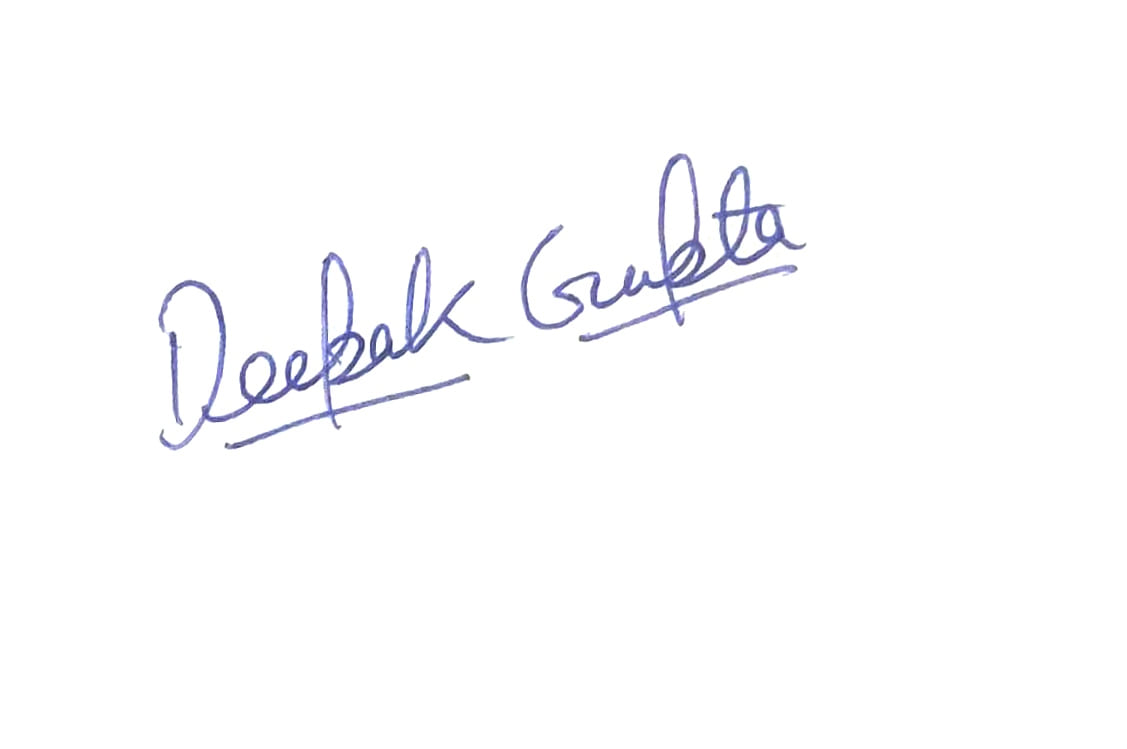
\includegraphics[width=4.5cm,trim=0 220 0 60,clip,keepaspectratio]{deepaksign.png}\\[-0.6em]%
	}{%
		\vspace*{1.2cm}%
	}%
	\rule{7.0cm}{0.5pt} \\
	\hspace{2pt}Name: Deepak Gupta \\
	\hspace{2pt}Roll No.: 2024PCS0024
\end{flushright}

\newpage
\thispagestyle{empty}
\cleardoublepage

%=========================================================
% Approval Sheet
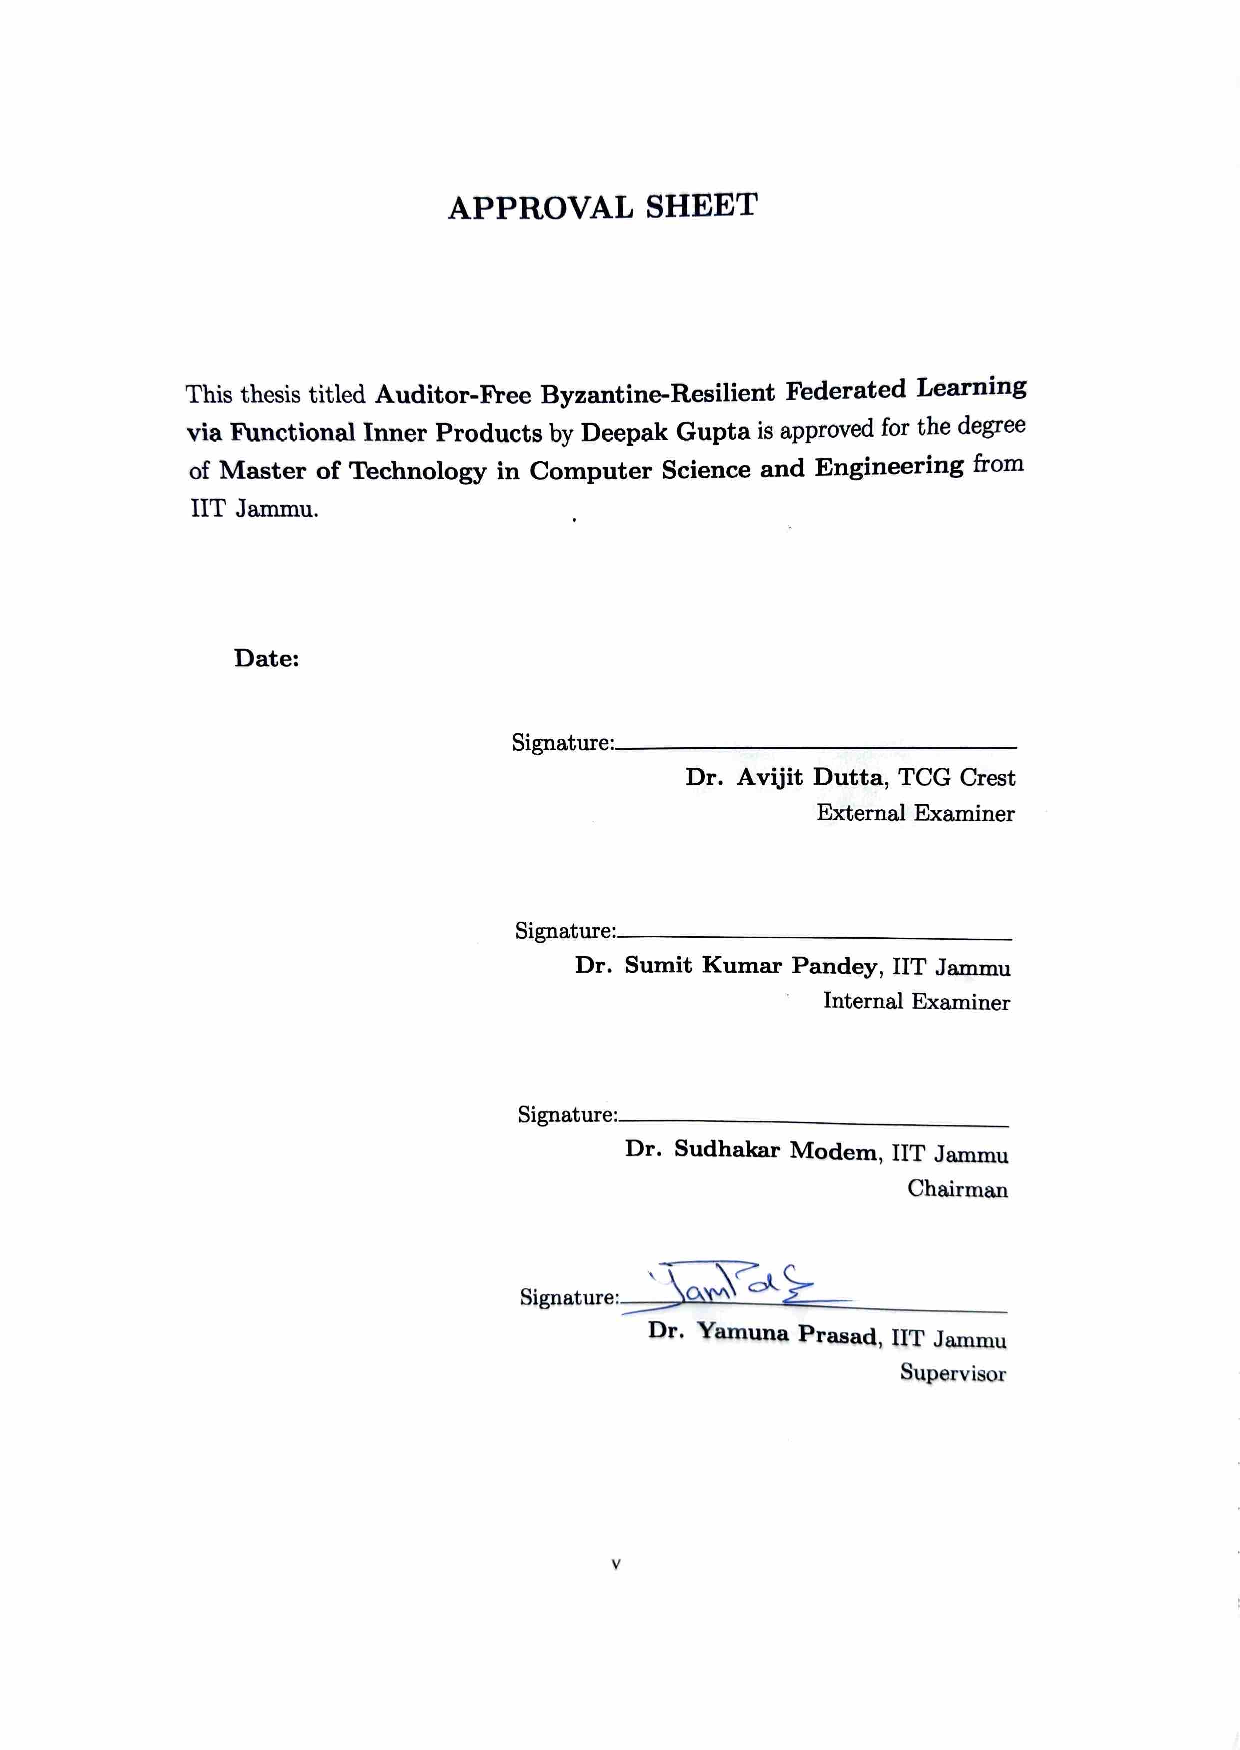
\includepdf[pages=1,pagecommand={\thispagestyle{empty}},width=\paperwidth,height=\paperheight,keepaspectratio]{approval_signed.pdf}

\newpage
\thispagestyle{empty}
\cleardoublepage

%=========================================================
% Dedication
\newpage
\thispagestyle{empty}
\vspace*{\fill}
\begin{center}
	\textit{\Large To my parents,}\\[0.4em]
	\textit{\Large who gave me the courage to dream big,}\\[0.4em]
	\textit{\Large and to my teachers,}\\[0.4em]
	\textit{\Large who showed me how to turn those dreams into reality.}
\end{center}
\vspace*{\fill}

\newpage
\thispagestyle{empty}
\cleardoublepage

%=========================================================
% Acknowledgement
\newpage
\thispagestyle{plain}
\begin{center}
\textbf{\Large Acknowledgement}
\end{center}

I want to record my thanks to the people who helped this dissertation reach its present form. The work passed through many small phases (problem reading, protocol drafts, experiment runs, and long revision cycles), and each of those phases was made easier by someone around me.

My deepest thanks go to my supervisor, Dr.~Yamuna~Prasad, Head of the Department of Computer Science and Engineering at IIT Jammu. Three areas feed into this thesis: privacy-preserving federated learning, applied cryptography, and adversarial machine learning. I genuinely do not think I could have tied them together without his guidance. Whatever coherence the final work has is in large part his doing. He let me follow my own ideas, but he rarely let a loose assumption pass; more than once he sent me back to justify a step or to repair a proof I had thought was finished. I learned a lot from working with him, as much from his patience as from the standard he sets for the work.

I am grateful, too, to the M.Tech and Ph.D. scholars at IIT Jammu who shared the lab and many long evenings with me. Whiteboard arguments, bugs we traced down together, and unhurried research conversations all helped shape parts of this work, and the months of writing and revision were a good deal less solitary for them.

The Department of Computer Science and Engineering at IIT Jammu provided the academic atmosphere, coursework, and the compute that this study needed; I thank the department, and all the faculty who taught me during the first year, for that support.

Finally, my parents and my family have stood behind me through every phase of this thesis; to them I owe far more than a line in an acknowledgement.

\vspace*{2mm}
\begin{flushright}
	\textbf{Deepak Gupta}
\end{flushright}

\newpage
\thispagestyle{empty}
\cleardoublepage

%=========================================================
% List of Publications (after Acknowledgement)
\newpage
\thispagestyle{plain}
\addcontentsline{toc}{chapter}{List of Publications}
\begin{center}
\textbf{\Large List of Publications}
\end{center}

\vspace{0.5cm}

\noindent \textbf{\large Conference Publications}
\begin{enumerate}
	\item Mahendra Kumar Gurve, Deepak Gupta, Nitin, and Yamuna Prasad, ``Eliminating the Auditor: Functional Inner Product Based Byzantine-Resilient Federated Learning,'' accepted as a poster at the \textit{ACM/IEEE International Conference on Embedded Artificial Intelligence and Sensing Systems (SenSys~2026)}, Saint-Malo, France, May 2026.
\end{enumerate}

\newpage
\thispagestyle{empty}
\cleardoublepage

	\addcontentsline{toc}{chapter}{Abstract}
	% Abstract page
\thispagestyle{plain}
\begin{center}
	\textbf{\Large Abstract}
\end{center}

\begingroup
\onehalfspacing
\setlength{\parskip}{6pt}

Federated Learning, or FL, lets many clients jointly fit one model without sending their raw data anywhere. To tighten the privacy story, recent work wraps every client update in an additive homomorphic cipher, giving the family known as Privacy-Preserving Federated Learning (PPFL). The catch is that the same cipher which keeps a curious server out of the gradients also keeps the server from telling honest clients apart from bad ones. A Byzantine client can simply flip its labels and silently push the global model in a wrong direction, pulling accuracy down or planting a back-door on one chosen class.

Most defences here bring in an auditor: a trusted third party that decrypts cluster-level statistics of the incoming updates and screens out the bad ones with distributional models. They work, but at a price. The auditor is itself a new trust anchor, the very thing PPFL was meant to remove. Decrypting cluster summaries also leaks structural information about the gradients, and the cubic covariance step makes cost grow much faster than $d$. A defence that is at once fully encrypted, free of any extra trust anchor, and linear in $d$ has so far been missing.

Functional Inner Product--Federated Learning, the framework developed in this thesis, is built around one idea: the verifier never needs to see a raw gradient. Working entirely under Paillier encryption, it computes one projection score per client: the Functional Inner Product (FIP) of that client's update against a fixed bootstrap reference direction. Once the FIP scalar is decrypted, the bootstrap audit is applied. The chapters that follow analyse this protocol along three axes: how much a scalar score actually reveals about the gradient, what region of update-space is still open to an attacker, and whether descent is preserved when the loss is $L$-smooth.

I built the framework end-to-end and ran it on MNIST and KDDCup99, with both IID and non-IID client splits, and with targeted and untargeted label-flipping attacks at malicious-client rates up to fifty percent. Across this grid, FIP-FL stays robust without any external auditor.

\endgroup

\newpage
\thispagestyle{empty}
\cleardoublepage

	\cleardoublepage
	\CompactFrontMatterList{\tableofcontents}
	\cleardoublepage
	\addcontentsline{toc}{chapter}{List of Figures}
	\CompactFrontMatterList{\listoffigures}
	\cleardoublepage
	\addcontentsline{toc}{chapter}{List of Tables}
	\CompactFrontMatterList{\listoftables}
	\cleardoublepage

	\addcontentsline{toc}{chapter}{List of Abbreviations}
	\begingroup
	\singlespacing
	\setlength{\parskip}{0pt}
	\noindent\textbf{\LARGE List of Abbreviations}
	\vspace{0.45cm}
	\small
	\begin{description}
		\setlength{\itemsep}{1pt}
		\setlength{\parsep}{0pt}
		\setlength{\topsep}{0pt}
		\item \textbf{ACC} \, - Overall Accuracy
		\item \textbf{BFV} \, - Brakerski--Fan--Vercauteren (homomorphic encryption scheme)
		\item \textbf{BGV} \, - Brakerski--Gentry--Vaikuntanathan (homomorphic encryption scheme)
		\item \textbf{CKKS} \, - Cheon--Kim--Kim--Song (approximate homomorphic encryption)
		\item \textbf{DCR} \, - Decisional Composite Residuosity
		\item \textbf{DoS} \, - Denial of Service
		\item \textbf{DP} \, - Differential Privacy
		\item \textbf{FedAvg} \, - Federated Averaging
		\item \textbf{FHE} \, - Fully Homomorphic Encryption
		\item \textbf{FIP} \, - Functional Inner Product
		\item \textbf{FIP-FL} \, - Functional Inner Product Federated Learning (proposed framework)
		\item \textbf{FL} \, - Federated Learning
		\item \textbf{FPR} \, - False Positive Rate
		\item \textbf{GMM} \, - Gaussian Mixture Model
		\item \textbf{HE} \, - Homomorphic Encryption
		\item \textbf{IID} \, - Independent and Identically Distributed
		\item \textbf{KDD} \, - Knowledge Discovery in Databases
		\item \textbf{MNIST} \, - Modified National Institute of Standards and Technology (database)
		\item \textbf{$O_{\text{acc}}$} \, - Other-label Accuracy
		\item \textbf{PCA} \, - Principal Component Analysis
		\item \textbf{PPFL} \, - Privacy-Preserving Federated Learning
		\item \textbf{R2L} \, - Remote-to-Local (KDDCup attack class)
		\item \textbf{SenSys} \, - ACM/IEEE International Conference on Embedded Artificial Intelligence and Sensing Systems
		\item \textbf{SGD} \, - Stochastic Gradient Descent
		\item \textbf{SHA} \, - Secure Hash Algorithm
		\item \textbf{SMPC} \, - Secure Multiparty Computation
		\item \textbf{$T_{\text{acc}}$} \, - Target-class Accuracy
		\item \textbf{TF-IDF} \, - Term Frequency -- Inverse Document Frequency
		\item \textbf{TKA} \, - Trusted Key Authority
		\item \textbf{TPR} \, - True Positive Rate
		\item \textbf{U2R} \, - User-to-Root (KDDCup attack class)
	\end{description}
	\endgroup

	\newpage
	\thispagestyle{empty}
	\cleardoublepage


	%	\usepackage{pdflscape}
	% Main thesis section
	\pagenumbering{arabic}
	\fancypagestyle{plain}{%
		\fancyhf{}%
		\fancyfoot[C]{\small\thepage}%
		\renewcommand{\headrulewidth}{0pt}%
		\renewcommand{\footrulewidth}{0pt}%
	}
	\pagestyle{thesismain}
	\chapter{Introduction}
\label{Intro:chap:chap1}
\graphicspath{{10.Chapter1/Images/}}

\section{Background and Context}

Federated Learning, FL for short, was put forward by McMahan and his coauthors~\cite{mcmahan2017communication} as a way of training a single global model without ever pulling the raw data into one place. The clients keep their samples on their own devices and send back only a gradient or a parameter update. That property is what makes the FL recipe useful for things like mobile keyboards, medical records, fraud-detection feeds, and anywhere else that the data is sensitive and naturally distributed.

But keeping the data local is, by itself, not really enough. The shared gradients can still leak training samples~\cite{zhu2019deep}, leak membership, or leak distributional traits of the underlying records. The line of work that hardens this channel is called Privacy-Preserving Federated Learning, or PPFL. In privacy-preserving federated learning, three ideas keep coming up: differential privacy, secure aggregation, and homomorphic encryption. My work sits squarely in the third camp. By choosing additive homomorphic encryption, I let the server add together encrypted model updates while never seeing an individual gradient in plain text.

\section{The Research Gap}

That strong privacy shield has a flipside. Once every update reaches the server as ciphertext, the usual checks for bad behaviour stop working. A single dishonest client can flip labels, stretch its gradients, or inject a poison vector, and the server cannot tell. Well-known robust rules such as Krum~\cite{blanchard2017machine}, the coordinate-wise median, the trimmed mean~\cite{yin2018byzantine}, and Bulyan~\cite{guerraoui2018hidden} all need plaintext inputs. Detectors like Auror~\cite{shen2016auror}, FL-Trust~\cite{cao2021fltrust}, and PEFL~\cite{liu2021privacy} face the same roadblock because they rely on gradients they can read.

The most relevant baseline that does work over encrypted gradients is the auditor-based scheme of Yazdinejad et al.~\cite{yazdinejad2024robust}. It is effective. But it depends on a trusted auditor, it decrypts cluster-level summaries to make decisions, it carries an $\mathcal{O}(d^3)$ covariance-inversion cost, and under non-IID partitions it exposes structural population information. The piece that is genuinely missing in the literature, then, is a defence that is at once auditor-free, robust, linear in $d$, and still usable when the federation is realistically heterogeneous.

\section{Research Objectives and Contributions}

What this thesis sets out to do is design, analyse, and evaluate FIP-FL, a Byzantine-resilient PPFL framework in which no auditor is involved. The verifier looks at each encrypted client update through a single functional inner product (FIP) against a fixed bootstrap reference direction; only one scalar per client per round ever needs to be decrypted. That scalar is then put through a bootstrap audit.

The main contributions of the thesis are the following.
\begin{enumerate}
    \item \textbf{An auditor-free PPFL architecture.} FIP-FL drops the external auditor entirely and does its verification straight on the ciphertexts, using a scalar FIP score.
    \item \textbf{A bootstrap audit.} The direction test discards the updates that point the wrong way, and after borderline restoration the audit rejects the lowest-scoring clients according to the attack-rate setting.
    \item \textbf{Formal guarantees.} The thesis proves scalar-gradient privacy, gives the admissibility region left to an attacker, derives monotone descent under $L$-smoothness, and shows lower verifier complexity than the auditor-based baseline.
    \item \textbf{Empirical validation.} FIP-FL is run on MNIST and on KDDCup99, under both IID and non-IID partitions, against targeted and untargeted label flipping, and with the malicious-client rate swept all the way to $50\%$.
    \item \textbf{Engineering efficiency.} The verifier ends up running in $\mathcal{O}(Nd+N\log N)$, in place of an $\mathcal{O}(d^3)$ covariance step, and parallelising Phase~II gives roughly a $13\times$ wall-clock speed-up on 25 cores.
\end{enumerate}

The research underlying this thesis has been accepted as a poster at the ACM/IEEE International Conference on Embedded Artificial Intelligence and Sensing Systems (SenSys~2026), Saint-Malo, France, May 2026.

	\chapter{Background and Motivation}
\label{Background:chap:chap2}
\graphicspath{{11.Chapter2/Images/}}

\section{Federated Learning and FedAvg}

Take $N$ clients. Client $i$ holds private data $\mathcal{D}_i=\{(x_k^{(i)},y_k^{(i)})\}_{k=1}^{n_i}$, and the total sample count is $n=\sum_i n_i$. The federated objective is then the size-weighted empirical risk
\begin{equation}
    F(\mathbf{w})=\sum_{i=1}^{N}\frac{n_i}{n}F_i(\mathbf{w}),\qquad
    F_i(\mathbf{w})=\frac{1}{n_i}\sum_{k=1}^{n_i}\ell(f_{\mathbf{w}}(x_k^{(i)}),y_k^{(i)}).
\end{equation}
The FedAvg algorithm of McMahan et al.~\cite{mcmahan2017communication} attacks this objective in the obvious way: send $\mathbf{w}^{(t)}$ down to every client, let each client run local SGD on its own shard, and average back what comes up. Writing the descent direction submitted by client $i$ as $\Delta\boldsymbol{\theta}_i^{(t)}=\mathbf{w}^{(t)}-\mathbf{w}_i^{(t+1)}$, the server step boils down to
\begin{equation}
    \mathbf{w}^{(t+1)}=\mathbf{w}^{(t)}-\sum_{i=1}^{N}\frac{n_i}{n}\Delta\boldsymbol{\theta}_i^{(t)}.
\end{equation}
So the server is left with a coordinate-wise weighted sum, and the raw samples themselves never have to move.

\section{IID and Non-IID Federations}

Many FedAvg studies pretend every client sees the same data distribution. Real deployments are messier. Phones, clinics, and sensors each carry their own label mix and feature quirks. I focus on label skew, meaning a client only sees part of the label set. Honest gradients then point in different directions, so any defence must separate natural drift from a real attack.

\section{Privacy-Preserving Federated Learning}

Raw gradients leak more than most people realise. A curious server can rebuild samples or test membership~\cite{zhu2019deep}. Three main defences exist: differential privacy, secure aggregation, and homomorphic encryption. Differential privacy adds noise but also hides useful signal. Secure aggregation protects each update yet cannot drop a bad one before the sum~\cite{bonawitz2017practical}. Homomorphic schemes keep everything encrypted while still allowing limited math. Paillier~\cite{paillier1999public} handles addition and scaling cheaply; BFV and CKKS~\cite{cheon2017homomorphic} support richer operations at a higher cost. I go with Paillier because my audit is simple: measure each encrypted update against a public reference vector through an inner product, all in linear time.

\section{Poisoning Attack Taxonomy}

\nocite{bhagoji2019analyzing}
I look at two label-flipping tricks. The untargeted version cycles every label and drags overall accuracy down. The targeted one maps a single source class to a target class and hurts that prediction. I leave out sign flips, scaling, model replacement, backdoors~\cite{bagdasaryan2020backdoor}, and collusion, though my audit still checks the direction and size of every update to keep those threats in mind.

	\chapter{Literature Survey}
\label{Literature:chap:chap3}
\graphicspath{{12.Chapter3/Images/}}

\section{Robust Aggregation Rules}
\label{sec:lit-aggreg}

Some defences swap the mean for sturdier estimators. Krum and Multi-Krum~\cite{blanchard2017machine} pick updates close to many neighbours but need every pairwise distance and cost $\mathcal{O}(N^{2}d)$. The coordinate-wise median and trimmed mean~\cite{yin2018byzantine} cut that to $\mathcal{O}(Nd\log N)$ yet struggle when genuine data vary strongly.

\section{Detection-Based Defences}
\label{sec:lit-detect}

Other methods try to catch bad clients first. Most still need plaintext. PEFL~\cite{liu2021privacy} works on ciphertext but slows down when attacks rise or data skew deepens~\cite{yazdinejad2024robust}. FoolsGold~\cite{fung2020limitations} tracks long-term similarity, while ShieldFL~\cite{ma2022shieldfl} brings in a helper. Strong detection often means plaintext, a trusted partner, or extra bandwidth. My approach avoids all three by releasing just one scalar per client.

\section{Auditor-Based PPFL Baseline}
\label{sec:lit-auditor}

Yazdinejad and colleagues~\cite{yazdinejad2024robust} add a trusted auditor who decrypts cluster summaries, fits a Gaussian mixture, and drops outliers with Mahalanobis distance before homomorphic averaging. They reach about $96.5$ percent target-class accuracy on non-IID MNIST under a fifty-percent flip, but that success requires an extra trust anchor, $\mathcal{O}(d^{3})$ covariance inversion, and leaking cluster stats.

\section{Positioning of FIP-FL}
\label{sec:lit-position}

My method, FIP-FL, keeps every update encrypted, calls on no auditor, swaps clustering for a simple alignment check, and stays linear in the model dimension $d$. The goal is straightforward: hold privacy tight while keeping Byzantine screening light.

	\chapter{Preliminaries}
\label{Preliminaries:chap:chap4}
\graphicspath{{13.Chapter4/Images/}}

\section{Notation}
\label{sec:prelim-notation}

Scalars are lowercase italics ($a$, $\eta$), vectors are lowercase bold ($\mathbf{x}$, $\boldsymbol{\theta}$), and matrices are uppercase bold ($\mathbf{W}$, $\mathbf{M}$). For $\mathbf{a},\mathbf{b}\in\mathbb{R}^{d}$,
\begin{equation}
    \langle \mathbf{a},\mathbf{b}\rangle=\sum_{k=1}^{d}a_kb_k,\qquad
    \|\mathbf{a}\|_2=\sqrt{\langle \mathbf{a},\mathbf{a}\rangle}.
\end{equation}
A Paillier ciphertext is written $[\![m]\!]=\mathrm{Enc}_{pk}(m)$. The main FL symbols are $N$ clients, model dimension $d$, round index $t$, local epochs $E$, batch size $B$, learning rate $\eta$, and Paillier security parameter $\lambda$.

\section{The Paillier Cryptosystem}
\label{sec:prelim-paillier}

The additive homomorphic scheme my implementation rests on is Paillier~\cite{paillier1999public}. Fix a security parameter $\lambda$. The Trusted Key Authority then draws two primes $p$ and $q$, sets $n=pq$, takes the generator $g=n+1$, and locks away the secret key $sk=(\ell,\alpha)$ with $\ell=\mathrm{lcm}(p-1,q-1)$ and $\alpha=\ell^{-1}\bmod n$. Throughout the thesis every experiment fixes $\lambda=1024$.

For plaintext $m\in\mathbb{Z}_n$ and random $r\in\mathbb{Z}_n^*$,
\begin{equation}
    \mathrm{Enc}_{pk}(m)=g^mr^n \pmod{n^2},
    \label{eq:paillier-enc}
\end{equation}
and decryption is
\begin{equation}
    \mathrm{Dec}_{sk}(c)=L(c^\ell\bmod n^2)\alpha \pmod n,\qquad L(x)=\frac{x-1}{n}.
    \label{eq:paillier-dec}
\end{equation}
For plaintexts $m_1,m_2$ and known integer $a$,
\begin{align}
    \mathrm{Enc}_{pk}(m_1)\mathrm{Enc}_{pk}(m_2)
        &\equiv \mathrm{Enc}_{pk}(m_1+m_2) \pmod{n^2}, \label{eq:paillier-add}\\
    \mathrm{Enc}_{pk}(m_1)^a
        &\equiv \mathrm{Enc}_{pk}(a m_1) \pmod{n^2}. \label{eq:paillier-mul}
\end{align}
Between them, these two identities cover everything FIP-FL ever asks for: encrypted sums and encrypted linear functionals. The protocol never once multiplies two ciphertexts together.

Gradients are real-valued, so before encryption they are turned into fixed-point integers. For a scale $s$,
\begin{equation}
    \mathrm{encode}(x)=\mathrm{round}(sx),\qquad
    \mathrm{decode}(z)=z/s.
    \label{eq:fixed-point}
\end{equation}
Signed values live inside the Paillier plaintext ring through centered modular encoding: a negative $-a$ is stored as $n-a$ and read back from the interval $(-n/2,n/2]$. Negative plaintext scalars that turn up during homomorphic multiplication are dealt with by modular inverses. The experiments fix $s=10{,}000$. One bookkeeping detail is worth flagging here: an encrypted FIP score multiplies an encoded update coordinate by an encoded reference coordinate, so once decrypted it has to be divided by $s^2$ to land back on the right scale.

\section{Functional Inner Product}
\label{sec:prelim-fip}

When the gradient vectors are flat real vectors, the Functional Inner Product used throughout this thesis is just the ordinary Euclidean dot product
\begin{equation}
    \langle \mathbf{g}_i,\mathbf{g}_{\mathrm{ref}}\rangle
        =\sum_{k=1}^{d}g_i^{(k)}g_{\mathrm{ref}}^{(k)}.
    \label{eq:fip-discrete}
\end{equation}
The name deliberately echoes inner-product functional encryption~\cite{abdalla2015simple}, which likewise reveals only an inner product of an otherwise hidden vector; in FIP-FL, however, that functional is realised through Paillier homomorphic operations rather than a dedicated functional-encryption scheme. In plain terms, the FIP score measures how well a client's gradient update aligns with the trusted reference direction, nothing more than that. Feed \eqref{eq:fip-discrete} into the Paillier identities for plaintext-scalar multiplication and ciphertext addition, and the score can be assembled entirely under encryption:
\begin{equation}
    [\![\langle \mathbf{g}_i,\mathbf{g}_{\mathrm{ref}}\rangle]\!]
    =
    \prod_{k=1}^{d}
    [\![g_i^{(k)}]\!]^{\,\mathrm{encode}(g_{\mathrm{ref}}^{(k)})}
    \pmod{n^2}.
    \label{eq:fip-homo}
\end{equation}
This lone scalar is the only thing ever decrypted, and even that step belongs to the TKA. Not a single coordinate of $\mathbf{g}_i$ is exposed anywhere in the round.

\section{System and Threat Model}
\label{sec:prelim-threat}

The FIP-FL protocol has four roles. The clients submit encrypted gradients. The Aggregation Server takes whatever ciphertexts the audit has accepted and broadcasts the new model. The FIP Verifier is the role that actually computes the scalar FIP scores and runs the bootstrap audit. The Trusted Key Authority (TKA) generates the Paillier keys and is allowed to decrypt only those scalar scores and aggregates that the protocol explicitly asks it to. The Verifier may be co-located with the server in practice; in either case, no external auditor enters the trust model.

The adversary in this thesis controls up to $f<N/2$ Byzantine clients. Such an adversary is free to relabel its own data, hand in any syntactically valid ciphertext it likes, coordinate with other malicious clients, and listen in on every public broadcast. The empirical part instantiates this model with targeted and untargeted label flipping, at malicious rates $f/N\in\{10\%,20\%,30\%,50\%\}$.

\section{Security and Privacy Goals}
\label{sec:prelim-goals}

The protocol is designed against four targets. \emph{Privacy}: neither the server nor the Verifier should learn any coordinate, norm, or pairwise distance over the client gradients beyond the scalar score $s_i^{(t)}=\langle\mathbf{g}_i^{(t)},\mathbf{g}_{\mathrm{ref}}^{(t)}\rangle$. \emph{Byzantine resilience}: an update is accepted only when it passes the bootstrap audit. \emph{Convergence}: the average of the accepted updates has to satisfy the descent-alignment plus step-size pair stated in Chapter~\ref{FIPFL:chap:chap5}. \emph{Efficiency}: the verifier should run in $\mathcal{O}(Nd+N\log N)$, and the aggregation step in $\mathcal{O}(|\mathcal{A}^{(t)}|d)$ for the accepted set $\mathcal{A}^{(t)}$.

	\begingroup
	\let\cleardoublepage\clearpage
	\chapter{Proposed Framework: FIP-FL}
\label{FIPFL:chap:chap5}
\graphicspath{{14.Chapter5/Images/}}

\section{System Architecture}
\label{sec:fip-arch}

FIP-FL is built around four logical roles: the $N$ clients, an Aggregation Server, a FIP Verifier, and a Trusted Key Authority (or TKA). In a single round, the clients put their Paillier ciphertexts on the wire, the Verifier turns each ciphertext into one alignment score, only the accepted ciphertexts make it to the aggregation server, and the TKA touches at most scalar scores or aggregate updates, never an individual plaintext gradient.

The system is organized so that each component has a clearly limited role. Clients perform local training and encrypt their updates. The Verifier evaluates these encrypted updates and filters suspicious ones. The server aggregates only the updates that pass the audit, while the TKA is responsible solely for the decryptions explicitly required by the protocol.

This separation is intentional. The Verifier can access encrypted client updates and the plaintext reference direction $\mathbf{R}^{(t)}$, but it never sees any individual gradient in plaintext form. Conversely, the TKA decrypts scalar FIP scores and aggregated updates, yet it has no access to the audit logic itself.

\section{System Setup and Key Distribution}
\label{sec:fip-setup}

The setup phase is executed only once, before round~1. As described in Algorithm~\ref{alg:fip-ppfl-init}, the protocol keeps the three forms of state deliberately separate. The cryptographic state is maintained by the TKA. The model state begins with a clean global model stored on the server. The geometric state, namely the unit-norm reference direction, is initialized using a small public bootstrap dataset and then stored at the Verifier.

\begin{algorithm}[t]
\caption{FIP-FL System Initialization and Reference Bootstrapping}
\label{alg:fip-ppfl-init}
\begin{algorithmic}[1]
\Require Number of clients $N$, model $f_{\boldsymbol{\theta}}$, public bootstrap set $\mathcal{D}_{\text{init}}$, security parameter $\lambda$, fixed-point scale $s$
\Ensure Registered clients, Paillier keys, initial global model $\boldsymbol{\theta}^{(0)}$, trusted reference direction $\mathbf{g}_{\text{ref}}^{(0)}$

\Statex \textbf{Key generation and registration}
\State $(pk, sk) \gets \textsc{PaillierKeyGen}(1^{\lambda})$ at the Trusted Key Authority
\State TKA keeps $sk$ sealed and releases only $pk$ to the clients and the FIP-FL server
\For{$i \gets 1$ \textbf{to} $N$}
    \State Register client $C_i$ and assign anonymous tag $\text{TagID}_i$
    \State Send $(pk, s)$ to client $C_i$
\EndFor

\Statex \textbf{Model and verifier initialisation}
\State Initialise global model parameters $\boldsymbol{\theta}^{(0)} \gets \mathbf{0}$
\State Broadcast $\boldsymbol{\theta}^{(0)}$ to all registered clients
\State Initialise encrypted-update table $\mathcal{U}^{(0)} \gets \emptyset$

\Statex \textbf{Reference bootstrapping}
\State Compute the trusted bootstrap gradient on public data:
\State $\widetilde{\mathbf{g}}_{\text{ref}}^{(0)} \gets \nabla_{\boldsymbol{\theta}}\mathcal{L}\!\left(f_{\boldsymbol{\theta}};\mathcal{D}_{\text{init}}\right)\big|_{\boldsymbol{\theta}=\boldsymbol{\theta}^{(0)}}$
\State Normalise the reference direction:
\State $\mathbf{g}_{\text{ref}}^{(0)} \gets \widetilde{\mathbf{g}}_{\text{ref}}^{(0)} / \max\!\left(\left\|\widetilde{\mathbf{g}}_{\text{ref}}^{(0)}\right\|_{2}, \varepsilon\right)$
\State Store $\mathbf{g}_{\text{ref}}^{(0)}$ at the FIP Verifier for round~$1$
\end{algorithmic}
\end{algorithm}

The public bootstrap set plays a role at exactly one point in the protocol: it gives us $\mathbf{g}_{\text{ref}}^{(0)}$ at the zero model. From round~$t\ge 1$ onwards we just call this reference direction $\mathbf{R}^{(t)}$.

\section{Per-Round Protocol}
\label{sec:fip-round}

After initialization, each round $t\ge 1$ follows the same core procedure described in the SenSys poster: encrypted gradient submission, FIP score computation, bootstrap-stage filtering, secure aggregation, and global model update.

\subsection{Phase I: Local Training and Encrypted Update Generation}
\label{sec:fip-phaseI}

In Phase~I, each client runs $E$ epochs of mini-batch SGD on its own shard, averages the gradients, flattens the weight and bias parameters into a single $d$-dimensional vector, encrypts each coordinate under Paillier, and ships the resulting ciphertext vector off to the Verifier. Algorithm~\ref{alg:fip-client-submit} writes out the honest version of this; a malicious client tampers with its labels before this step ever begins, so its arithmetic on the device is the same.

\begin{algorithm}[t]
\caption{Client-Side Local Training and Encrypted Gradient Submission}
\label{alg:fip-client-submit}
\begin{algorithmic}[1]
\Require Client $C_i$ with data $\mathcal{D}_i$, round model $\boldsymbol{\theta}^{(t)}$, public key $pk$, scale $s$, epochs $E$, batch size $B$, learning rate $\eta$
\Ensure Encrypted submission $\mathcal{M}_i^{(t)}$

\State $\boldsymbol{\theta}_{i} \gets \boldsymbol{\theta}^{(t)}$
\State $\mathbf{g}_{i}^{(t)} \gets \mathbf{0}$, $m_i \gets 0$
\For{$e \gets 1$ \textbf{to} $E$}
    \ForAll{mini-batches $\mathcal{B} \subset \mathcal{D}_i$ of size $B$}
        \State $\mathbf{h} \gets \nabla_{\boldsymbol{\theta}}\mathcal{L}\!\left(f_{\boldsymbol{\theta}_{i}};\mathcal{B}\right)$
        \State $\mathbf{g}_{i}^{(t)} \gets \mathbf{g}_{i}^{(t)} + \mathbf{h}$, $m_i \gets m_i + 1$
        \State $\boldsymbol{\theta}_{i} \gets \boldsymbol{\theta}_{i} - \eta \mathbf{h}$
    \EndFor
\EndFor
\State $\mathbf{g}_{i}^{(t)} \gets \mathbf{g}_{i}^{(t)} / \max(m_i,1)$
\State Flatten $\mathbf{g}_{i}^{(t)}$ into coordinates $\left(g_{i,1}^{(t)},\ldots,g_{i,d}^{(t)}\right)$
\For{$k \gets 1$ \textbf{to} $d$}
    \State $\widehat{g}_{i,k}^{(t)} \gets \textsc{Encode}_{s}\!\left(g_{i,k}^{(t)}\right)$
    \State $[\![g_{i,k}^{(t)}]\!] \gets \textsc{Enc}_{pk}\!\left(\widehat{g}_{i,k}^{(t)}\right)$
\EndFor
\State $\mathcal{M}_i^{(t)} \gets \left(\text{TagID}_i,\{[\![g_{i,k}^{(t)}]\!]\}_{k=1}^{d}\right)$
\State Send $\mathcal{M}_i^{(t)}$ to the FIP Verifier
\end{algorithmic}
\end{algorithm}

\subsection{Phase II: Homomorphic FIP Score Computation}
\label{sec:fip-phaseII}

In Phase~II, the Verifier forms the projection of the client update onto $\mathbf{R}^{(t)}$ \emph{while the update itself is still in ciphertext form}. The Paillier identities for plaintext-scalar multiplication and ciphertext addition take care of the inner product. After this is done, only the scalar $s_i^{(t)}=\langle \mathbf{g}_i^{(t)},\mathbf{R}^{(t)}\rangle$ ever gets handed to the TKA for decryption; the individual coordinates of $\mathbf{g}_i^{(t)}$ stay sealed. Algorithm~\ref{alg:fip-score} writes this out step by step.

\begin{algorithm}[t]
\caption{Homomorphic Functional Inner Product Score Computation}
\label{alg:fip-score}
\begin{algorithmic}[1]
\Require Encrypted submissions $\mathcal{U}^{(t)}$, reference $\mathbf{R}^{(t)}$, public key $pk$, secret key $sk$ held by TKA, scale $s$
\Ensure FIP score map $\mathcal{S}^{(t)}$

\State $\mathcal{S}^{(t)} \gets \emptyset$
\State Encode reference coordinates $\widehat{R}_{k}^{(t)} \gets \textsc{Encode}_{s}\!\left(R_{k}^{(t)}\right)$ for $k=1,\ldots,d$
\ForAll{$\left(\text{TagID}_i,\{[\![g_{i,k}^{(t)}]\!]\}_{k=1}^{d}\right) \in \mathcal{U}^{(t)}$}
    \State $[\![\widehat{s}_{i}^{(t)}]\!] \gets \textsc{Enc}_{pk}(0)$
    \For{$k \gets 1$ \textbf{to} $d$}
        \State $[\![\widehat{s}_{i}^{(t)}]\!] \gets [\![\widehat{s}_{i}^{(t)}]\!] \cdot \left([\![g_{i,k}^{(t)}]\!]\right)^{\widehat{R}_{k}^{(t)}} \bmod n^{2}$
    \EndFor
    \State Send $[\![\widehat{s}_{i}^{(t)}]\!]$ to TKA for scalar decryption
    \State $\widehat{s}_{i}^{(t)} \gets \textsc{Dec}_{sk}\!\left([\![\widehat{s}_{i}^{(t)}]\!]\right)$
    \State $s_i^{(t)} \gets \textsc{Decode}_{s^{2}}\!\left(\widehat{s}_{i}^{(t)}\right)$
    \State $\mathcal{S}^{(t)}[\text{TagID}_i] \gets s_i^{(t)}$
\EndFor
\State \Return $\mathcal{S}^{(t)}$
\end{algorithmic}
\end{algorithm}

\subsection{Phase III: Adaptive Bootstrap-Only Stage-1 Audit}
\label{sec:fip-phaseIII}

The audit begins with a direction test on the bootstrap FIP scores. Clients whose scores exceed the direction threshold are accepted, while the remaining clients are placed in a rejected set. If this initial pass leaves too few accepted clients, borderline rejected clients are restored within a noise-aware band around the threshold.

The final step uses the attack-rate setting to keep only the lowest-scoring rejected clients. All other rejected clients are restored to the accepted set. The complete bootstrap-stage procedure is given in Algorithm~\ref{alg:stage1_audit}.

\begin{algorithm}[t]
\caption{Adaptive Bootstrap-Only Stage-1 Audit}
\label{alg:stage1_audit}
\begin{algorithmic}[1]
\Require Bootstrap FIP scores $S^{(t)}$, direction threshold $\epsilon_{\mathrm{dir}}$, attack-rate setting $\rho$, noise scale $\sigma_{\mathrm{noise}}$
\Ensure Accepted set $\mathcal{A}^{(t)}$, rejected set $\mathcal{R}^{(t)}$

\State $\mathcal{A}^{(t)} \gets \emptyset$
\State $\mathcal{R}^{(t)} \gets \emptyset$

\ForAll{$\left(\text{TagID}_i,s_i^{(t)}\right) \in S^{(t)}$}
    \If{$s_i^{(t)} > \epsilon_{\mathrm{dir}}$}
        \State $\mathcal{A}^{(t)} \gets \mathcal{A}^{(t)} \cup \{\text{TagID}_i\}$
    \Else
        \State $\mathcal{R}^{(t)} \gets \mathcal{R}^{(t)} \cup \{\text{TagID}_i\}$
    \EndIf
\EndFor

\State $K_{\min} \gets \left\lceil 0.5N \right\rceil$
\State $\delta_R \gets \max\!\left(3\cdot\sigma_{\mathrm{noise}},\,0.03\right)$

\While{$|\mathcal{A}^{(t)}| < K_{\min}$}
    \State Select $C_j \in \mathcal{R}^{(t)}$ with the largest bootstrap score
    \If{$\left|s_j^{(t)}-\epsilon_{\mathrm{dir}}\right| \le \delta_R$}
        \State $\mathcal{A}^{(t)} \gets \mathcal{A}^{(t)} \cup \{C_j\}$
        \State $\mathcal{R}^{(t)} \gets \mathcal{R}^{(t)} \setminus \{C_j\}$
    \Else
        \State \textbf{break}
    \EndIf
\EndWhile

\State $B \gets \mathrm{round}(\rho N)$
\State Sort $\mathcal{R}^{(t)}$ in ascending order of bootstrap score
\State $\mathcal{R}_{\mathrm{keep}}^{(t)} \gets$ the $B$ lowest-score rejects in $\mathcal{R}^{(t)}$
\State $\mathcal{A}^{(t)} \gets \mathcal{A}^{(t)} \cup \left(\mathcal{R}^{(t)}\setminus\mathcal{R}_{\mathrm{keep}}^{(t)}\right)$
\State $\mathcal{R}^{(t)} \gets \mathcal{R}_{\mathrm{keep}}^{(t)}$

\State \Return $\mathcal{A}^{(t)},\mathcal{R}^{(t)}$
\end{algorithmic}
\end{algorithm}

\subsection{Phase IV: Secure Aggregation}
\label{sec:fip-phaseIV}

Phase~IV is short. The ciphertexts that the audit rejected are simply dropped; they are never decrypted at all. Whatever survives is folded into one pooled encrypted sum, and only that sum is later opened.

\subsection{Phase V: Model Update and Distribution}
\label{sec:fip-phaseV}

In Phase~V, the server updates the global model using the averaged accepted gradient. The server decrypts only the aggregate update, never an individual client update. If all client updates are rejected in a given round, the current model is carried forward unchanged to the next round.

Algorithm~\ref{alg:secure_aggregation} presents secure aggregation and model update together in a single procedure. The bootstrap reference remains fixed during this step.

\begin{algorithm}[t]
\caption{Secure Aggregation and Model Update}
\label{alg:secure_aggregation}
\begin{algorithmic}[1]
\Require Accepted encrypted set $\mathcal{A}^{(t)}$, model $\boldsymbol{\theta}^{(t)}$, public key $pk$, secret key $sk$, fixed-point scale $s$, learning rate $\eta$
\Ensure Updated model $\boldsymbol{\theta}^{(t+1)}$

\If{$\mathcal{A}^{(t)}=\emptyset$}
    \State $\boldsymbol{\theta}^{(t+1)} \gets \boldsymbol{\theta}^{(t)}$
    \State Broadcast $\boldsymbol{\theta}^{(t+1)}$
    \State \Return $\boldsymbol{\theta}^{(t+1)}$
\EndIf

\State $m \gets |\mathcal{A}^{(t)}|$

\For{$k \gets 1$ \textbf{to} $d$}
    \State $[\![\widehat{G}_{k}^{(t)}]\!] \gets \textsc{Enc}_{pk}(0)$
    \ForAll{$\left(\text{TagID}_i,\{[\![g_{i,\ell}^{(t)}]\!]\}_{\ell=1}^{d}\right) \in \mathcal{A}^{(t)}$}
        \State $[\![\widehat{G}_{k}^{(t)}]\!] \gets [\![\widehat{G}_{k}^{(t)}]\!] \cdot [\![g_{i,k}^{(t)}]\!] \bmod n^{2}$
    \EndFor
    \State Send $[\![\widehat{G}_{k}^{(t)}]\!]$ to TKA for aggregate decryption
    \State $\widehat{G}_{k}^{(t)} \gets \textsc{Dec}_{sk}\!\left([\![\widehat{G}_{k}^{(t)}]\!]\right)$
    \State $g_{\text{global},k}^{(t)} \gets \textsc{Decode}_{s}\!\left(\widehat{G}_{k}^{(t)}\right)/m$
\EndFor

\State $\boldsymbol{\theta}^{(t+1)} \gets \boldsymbol{\theta}^{(t)}-\eta\mathbf{g}_{\text{global}}^{(t)}$
\State Broadcast $\boldsymbol{\theta}^{(t+1)}$
\Comment{Bootstrap reference remains fixed}
\State \Return $\boldsymbol{\theta}^{(t+1)}$
\end{algorithmic}
\end{algorithm}

\section{Theoretical Analysis}
\label{sec:fip-theory}

The three theorems collected below match, one to one, the four design targets stated in Section~4.5 (privacy, Byzantine resilience, and convergence; the efficiency target is a complexity statement and is read off directly from the algorithms above).

\subsection{Gradient Privacy}

\begin{theorem}[Gradient Privacy]
\label{thm:fip-privacy}
In every round $t$, the FIP Verifier reveals exactly one scalar per client, namely the projection $s_i^{(t)} = \langle \mathbf{g}_i^{(t)}, \mathbf{R}^{(t)} \rangle \in \mathbb{R}$. For a gradient of dimension $d \gg 1$, recovering $\mathbf{g}_i^{(t)}$ from $s_i^{(t)}$ is information-theoretically impossible: the linear system $\mathbf{R}^{(t)\top}\mathbf{g}_i^{(t)} = s_i^{(t)}$ is under-determined and admits a $(d-1)$-dimensional affine solution space. Equivalently, the mutual information satisfies $I(\mathbf{g}_i^{(t)}; s_i^{(t)}) \le H(s_i^{(t)}) \ll H(\mathbf{g}_i^{(t)})$.
\end{theorem}

\begin{proof}
The FIP Verifier's only operation on ciphertext $[\![\mathbf{g}_i^{(t)}]\!]$ is the homomorphic inner product of \eqref{eq:fip-homo}, which yields $[\![s_i^{(t)}]\!]$. Given $s_i^{(t)}$ and $\mathbf{R}^{(t)}$, the preimage of $\mathbf{g}\mapsto\langle\mathbf{g},\mathbf{R}^{(t)}\rangle$ is a $(d-1)$-dimensional affine hyperplane. Gradients differing by a vector orthogonal to $\mathbf{R}^{(t)}$ are indistinguishable from the scalar alone, and the data-processing inequality gives $I(\mathbf{g}_i^{(t)}; s_i^{(t)}) \le H(s_i^{(t)}) \ll H(\mathbf{g}_i^{(t)})$.
\end{proof}

\subsection{Attack Resilience}

\begin{theorem}[Bootstrap Audit Rejection Rule]
\label{thm:fip-security}
In every round $t$, the audit of Algorithm~\ref{alg:stage1_audit} rejects exactly the $B=\mathrm{round}(\rho N)$ lowest-scoring clients among those whose bootstrap FIP scores remain below the direction threshold $\epsilon_{\mathrm{dir}}$ after borderline restoration; every other client is accepted. In particular, a direction-reversing update of the form $\mathbf{g}_{\text{adv}}\approx-\mathbf{g}_{\text{honest}}$ produces a score below $\epsilon_{\mathrm{dir}}$ and, lying among the lowest scores, is rejected, while the audit process remains independent of any external auditor.
\end{theorem}

\begin{proof}
The claim follows directly from the steps of Algorithm~\ref{alg:stage1_audit}. The direction test places every client with $s_i^{(t)}>\epsilon_{\mathrm{dir}}$ in the accepted set $\mathcal{A}^{(t)}$ and every other client in the rejected set $\mathcal{R}^{(t)}$. If $|\mathcal{A}^{(t)}|<K_{\min}$, borderline clients whose scores lie within the noise-aware band $\delta_R$ of $\epsilon_{\mathrm{dir}}$ are restored to $\mathcal{A}^{(t)}$ in descending order of score. The algorithm then sorts $\mathcal{R}^{(t)}$ in ascending order of bootstrap score, keeps only the $B=\mathrm{round}(\rho N)$ lowest-scoring clients in the rejected set, and restores all remaining clients to $\mathcal{A}^{(t)}$. A direction-reversing update scores below $\epsilon_{\mathrm{dir}}$, falls outside the restoration band, and sits among the lowest-scoring entries of the sorted rejected set, so it is retained in $\mathcal{R}^{(t)}$ and never enters the aggregate.
\end{proof}

\subsection{Convergence Guarantee}

\begin{theorem}[Descent under $L$-Smoothness]
\label{thm:fip-convergence}
Let $F(\mathbf{w})$ be $L$-smooth, and let $\Delta_{\text{global}}^{(t)}$ denote the mean of the accepted updates in round $t$. If the accepted aggregate is aligned with the descent direction of the true gradient, that is,
\begin{equation}
    \langle \nabla F(\mathbf{w}^{(t)}),\, \Delta_{\text{global}}^{(t)} \rangle > 0,
\end{equation}
then any learning rate
\begin{equation}
    0 < \eta < \frac{2\langle \nabla F(\mathbf{w}^{(t)}),\, \Delta_{\text{global}}^{(t)} \rangle}{L\|\Delta_{\text{global}}^{(t)}\|_2^2}
\end{equation}
gives a strict one-round loss decrease:
\begin{equation}
    F(\mathbf{w}^{(t+1)}) < F(\mathbf{w}^{(t)}).
\end{equation}
Consequently, if this alignment holds in expectation over accepted rounds, the expected global loss decreases monotonically.
\end{theorem}

\begin{proof}
Starting from the $L$-smoothness descent lemma we get
\begin{equation}
    F(\mathbf{w}^{(t)}-\eta\Delta_{\text{global}}^{(t)})
    \le
    F(\mathbf{w}^{(t)})
    -\eta\langle\nabla F(\mathbf{w}^{(t)}),\Delta_{\text{global}}^{(t)}\rangle
    +\frac{L\eta^2}{2}\|\Delta_{\text{global}}^{(t)}\|_2^2 .
\end{equation}
The key idea is that the alignment assumption makes the linear term strictly negative, while the bound on $\eta$ ensures that the quadratic term does not dominate it. Under this step-size condition, the right-hand side remains strictly smaller than $F(\mathbf{w}^{(t)})$.

In practice, the FIP-FL filter is designed to make this assumption reasonable. Only updates passing the bootstrap audit are included in $\Delta_{\text{global}}^{(t)}$. Importantly, the theorem does not require the reference direction to equal the true gradient; it states the average descent condition that the accepted aggregate must satisfy.
\end{proof}

	\chapter{Experimental Setup}
\label{Setup:chap:chap6}
\graphicspath{{15.Chapter6/Images/}}

This chapter pins down the empirical setting in which FIP-FL is run: which datasets we use, how the data is split among the clients, what attack the adversary mounts, which numbers we look at, and the implementation and hardware stack that the experiments actually live on.

\section{Datasets}
\label{sec:setup-datasets}

The evaluation grid runs on two benchmarks --- one image task and one intrusion-detection task. The high-level statistics are listed in Table~\ref{tab:datasets}.

\begin{table}[H]
\centering
\caption{Datasets used in the evaluation of FIP-FL.}
\label{tab:datasets}
\begin{tabular}{@{}lcccc@{}}
\toprule
\textbf{Dataset} & \textbf{Modality} & \textbf{Classes} & \textbf{Features} & \textbf{Samples} \\
\midrule
MNIST           & Image   & 10 & $784$ & $60{,}000 / 10{,}000$ \\
KDDCup99        & Tabular & 5  & $41$  & $\approx 494$K ($10\%$) \\
\bottomrule
\end{tabular}
\end{table}

\noindent\textbf{MNIST.} The MNIST corpus has $60{,}000$ training and $10{,}000$ test grayscale images at $28\times28$, labelled over the digits $\{0,1,\ldots,9\}$. Every image is flattened to a $784$-dimensional vector and rescaled into the unit interval. The same dataset is the headline benchmark in Yazdinejad et al.~\cite{yazdinejad2024robust}, which makes it the direct comparison point against the auditor-based baseline.

\noindent\textbf{KDDCup99.} KDDCup99 is the canonical network-intrusion benchmark. The full archive contains around $4.9$ million labelled connection records; the experiments here use the standard $10\%$ subset, which is roughly $494{,}000$ records. Each record exposes $41$ features mixing traffic counters and protocol flags, and the labels are collapsed into five classes --- \textsc{Normal}, \textsc{DoS}, \textsc{Probe}, \textsc{R2L} and \textsc{U2R}. Categorical fields are one-hot encoded and every feature is standardised. The class distribution is strongly imbalanced, which is exactly what makes this dataset a useful stress test: it forces the audit to behave even when the priors are far from uniform.

\noindent\textbf{Model Architecture.} For both datasets, a single-layer softmax logistic regression classifier is used. This choice is consistent with the model used in the SenSys 2026 poster as well as the auditor-based baseline. The total number of parameters is $d=(\text{input dim})\cdot C+C$, where the final term corresponds to the bias.

A compact model is selected for two main reasons. First, Paillier encryption with $\lambda=1024$ bits is still practical when the parameter dimension remains in the range of a few thousand. Second, the convexity and $L$-smoothness assumptions required in Theorem~\ref{thm:fip-convergence} are naturally satisfied by softmax logistic regression. In contrast, for deep neural networks these assumptions would hold only approximately.

\section{Data Partitioning}
\label{sec:setup-partition}

Each dataset is sliced into $N=10$ disjoint client shards, and I run the experiments under two partition regimes. In the IID regime the training set is shuffled once and dealt out into equal-sized shards, so each client ends up with roughly $|\mathcal{D}_{\text{train}}|/N$ samples and the expected label histogram on every shard matches the global one.

For the non-IID regime I use label skew. With a $C$-class task, client $i$ gets a primary label set $\mathcal{L}_{i}\subset\{0,1,\ldots,C-1\}$ of size $\lceil C/2\rceil$, and the overlap between successive clients is $\lfloor C/4\rfloor$. The client data are assigned using an $80/20$ rule. For each client, $80\%$ of the data comes from its primary labels, while the remaining $20\%$ is sampled from the full training set. This partitioning strategy ensures that each client still retains a small number of samples from every class. The setup follows the evaluation protocol used in SenSys 2026 and is also similar to the non-IID configuration considered by Yazdinejad et al.~\cite{yazdinejad2024robust}.

At the same time, the partition is deliberately challenging because even honest clients may produce different descent directions. As a result, the audit mechanism must tolerate normal data heterogeneity while still being able to identify malicious updates reliably.

\section{Attack Models}
\label{sec:setup-attacks}

Two pre-training label-flipping attacks make up the empirical sweep. Neither needs the adversary to know anything about Paillier or about the FIP-FL audit logic; both are plain data-side manipulations.

\noindent\textbf{Untargeted label flipping.} A malicious client relabels each local sample by a fixed cyclic offset,
\begin{equation}
    y_{k}^{(i,\,\text{mal})} \;=\; (y_{k}^{(i)} + \kappa) \bmod C .
\end{equation}
On MNIST I take $\kappa=5$, which gives a no-fixed-point permutation of the ten digits, and on KDDCup99 I take $\kappa=2$ because the task only has five classes. The aim of this attack is to drag overall accuracy down by pulling each malicious client's local gradient toward a deliberately wrong classification objective.

\noindent\textbf{Targeted label flipping.} A malicious client touches only a single source class $c_s$ and remaps it to a chosen target class $c_t$,
\begin{equation}
    y_{k}^{(i,\,\text{mal})} \;=\; \begin{cases}
        c_{t} & \text{if } y_{k}^{(i)} = c_{s}, \\
        y_{k}^{(i)} & \text{otherwise.}
    \end{cases}
\end{equation}
On MNIST the chosen source--target pair is $(c_s,c_t)=(0,7)$, and on KDDCup99 I use the analogous pair drawn from the two classes that dominate in the skew regime. The point of this attack is to break one semantic class while leaving overall accuracy looking reasonable, so the relevant diagnostic metric is the target-class accuracy rather than the overall one.

\noindent\textbf{Malicious-client rates.} For every combination of dataset, partition and attack type, the malicious-client fraction is swept over $f/N\in\{10\%,20\%,30\%,50\%\}$. The $50\%$ row is the most demanding stress test, sitting right at the boundary that majority-based aggregation can in principle survive.

\section{Evaluation Metrics}
\label{sec:setup-metrics}

Five metrics are used in the experiments. Three of them evaluate model utility on held-out test data, while the remaining two measure how effectively the verifier distinguishes malicious clients from honest ones.

\noindent\textbf{Target accuracy (Tacc).} This metric evaluates performance only on test samples belonging to the targeted source class $c_s$:
\begin{equation}
    \mathrm{Tacc} \;=\; \frac{|\{(x, y) \in \mathcal{D}_{\text{test}} : y = c_{s},\; \hat{f}(x) = c_{s}\}|}{|\{(x, y) \in \mathcal{D}_{\text{test}} : y = c_{s}\}|}.
\end{equation}
A successful targeted attack reduces this value, whereas an effective defence keeps it close to the clean baseline. For untargeted attacks, class $0$ is taken as a fixed reference class so that results remain comparable across rows.

\noindent\textbf{Other-label accuracy (Oacc).} Other-label accuracy measures performance on all test samples whose labels are not $c_s$:
\begin{equation}
    \mathrm{Oacc} \;=\; \frac{|\{(x, y) \in \mathcal{D}_{\text{test}} : y \neq c_{s},\; \hat{f}(x) = y\}|}{|\{(x, y) \in \mathcal{D}_{\text{test}} : y \neq c_{s}\}|}.
\end{equation}
Together, $\mathrm{Tacc}$ and $\mathrm{Oacc}$ show whether the attack mainly affects the target class or also damages the rest of the task.

\noindent\textbf{Overall accuracy (ACC).} Overall accuracy is the standard test accuracy over all classes:
\begin{equation}
    \text{ACC} \;=\; \frac{|\{(x, y) \in \mathcal{D}_{\text{test}} : \hat{f}(x) = y\}|}{|\mathcal{D}_{\text{test}}|}.
\end{equation}
This is the main utility metric for untargeted attack experiments.

\noindent\textbf{True positive rate (TPR).} TPR is the fraction of malicious clients rejected by the FIP-FL audit:
\begin{equation}
    \mathrm{TPR} \;=\; \frac{|\{i : \text{client } i \text{ is malicious and rejected}\}|}{|\{i : \text{client } i \text{ is malicious}\}|}.
\end{equation}
A higher TPR means that fewer malicious clients pass through the verifier.

\noindent\textbf{False positive rate (FPR).} This is the fraction of honest clients that are wrongly rejected:
\begin{equation}
    \mathrm{FPR} \;=\; \frac{|\{i : \text{client } i \text{ is honest and rejected}\}|}{|\{i : \text{client } i \text{ is honest}\}|}.
\end{equation}
This metric captures the cost of filtering honest participants. All five metrics are averaged over three independent random seeds. Standard deviation is reported only when it is greater than $0.5$ percentage points.

\section{Implementation and Hardware}
\label{sec:setup-impl}

The implementation is written in Python~3. \texttt{NumPy} is used for linear algebra, \texttt{scikit-learn} provides the dataset loaders and feature pipelines, and Paillier encryption is implemented using the \texttt{phe} library with a $1024$-bit modulus. The FIP Verifier and Aggregation Server run as separate Python processes and communicate through in-memory queues. The clients are simulated as worker processes. Both encryption and the homomorphic inner-product computation are parallelised using \texttt{multiprocessing}.

The wall-clock results in Chapter~\ref{Comparison:chap:chap8} were measured on a Linux workstation with a $25$-core CPU and $128$~GB of RAM.

	\chapter{Results and Analysis}
\label{Results:chap:chap7}
\graphicspath{{16.Chapter7/Images/}}

This chapter goes through the empirical results of FIP-FL on the grid defined in Chapter~\ref{Setup:chap:chap6}. Each table reports the relevant round-300 numbers --- overall accuracy ($\text{ACC}$), target-class accuracy ($T_{\text{acc}}$), other-label accuracy ($O_{\text{acc}}$), the true positive rate (TPR), and the false positive rate (FPR). Accuracies are quoted as percentages, and TPR and FPR are quoted as proportions in $[0,1]$.

%=====================================================================
\section{Non-IID Partition, Untargeted Attacks}
\label{sec:res-nonIID-untarg}

Of the four non-IID rows, the untargeted one is in some ways the most demanding. The label skew has already pushed the honest-client gradients away from each other, and on top of that the malicious clients are sending in label-flipped gradients that genuinely point away from the descent direction. Overall accuracy is the right utility number to read here, with TPR and FPR sitting alongside it as the cost-of-filtering pair.

\subsection{MNIST}
\label{sec:res-nonIID-untarg-mnist}

\begin{table}[H]
\centering
\caption{MNIST, non-IID partition, untargeted label-flipping attack.}
\label{tab:res-nonIID-untarg-mnist}
\begin{tabular}{@{}cccccc@{}}
\toprule
\textbf{AR} & \textbf{ACC (\%)} & \textbf{$T_{\text{acc}}$ (\%)} & \textbf{$O_{\text{acc}}$ (\%)} & \textbf{TPR} & \textbf{FPR} \\
\midrule
10\% & 91.22 & 97.60 & 90.18 & 1.00 & 0.00 \\
20\% & 91.02 & 97.87 & 89.94 & 1.00 & 0.00 \\
30\% & 90.78 & 97.33 & 89.31 & 1.00 & 0.00 \\
50\% & 91.10 & 97.51 & 89.91 & 1.00 & 0.20 \\
\bottomrule
\end{tabular}
\end{table}

\subsection{KDDCup99}
\label{sec:res-nonIID-untarg-kdd}

\begin{table}[H]
\centering
\caption{KDDCup99, non-IID partition (Dirichlet $\alpha=0.5$), untargeted label-flipping attack.}
\label{tab:res-nonIID-untarg-kdd}
\begin{tabular}{@{}cccccc@{}}
\toprule
\textbf{AR} & \textbf{ACC (\%)} & \textbf{$T_{\text{acc}}$ (\%)} & \textbf{$O_{\text{acc}}$ (\%)} & \textbf{TPR} & \textbf{FPR} \\
\midrule
10\% & 99.71 & 99.50 & 84.62 & 1.00 & 0.00 \\
20\% & 99.72 & 99.55 & 83.65 & 1.00 & 0.00 \\
30\% & 99.69 & 99.45 & 85.58 & 1.00 & 0.14 \\
50\% & 99.69 & 99.70 & 77.88 & 1.00 & 0.40 \\
\bottomrule
\end{tabular}
\end{table}

\paragraph{Observations.} Across both datasets, FIP-FL ends up rejecting every single malicious update and the utility number stays close to its undefended-clean value even under the non-IID untargeted load. On MNIST the ACC sits between $90.78\%$ and $91.22\%$, and false rejection only kicks in once the attack rate hits $50\%$. On KDDCup99 the ACC remains above $99.6\%$ throughout the sweep, even at the point where the FPR begins to rise under the heaviest non-IID setting.

\begin{figure}[!htbp]
\centering
\subfigure[MNIST ACC trajectory]{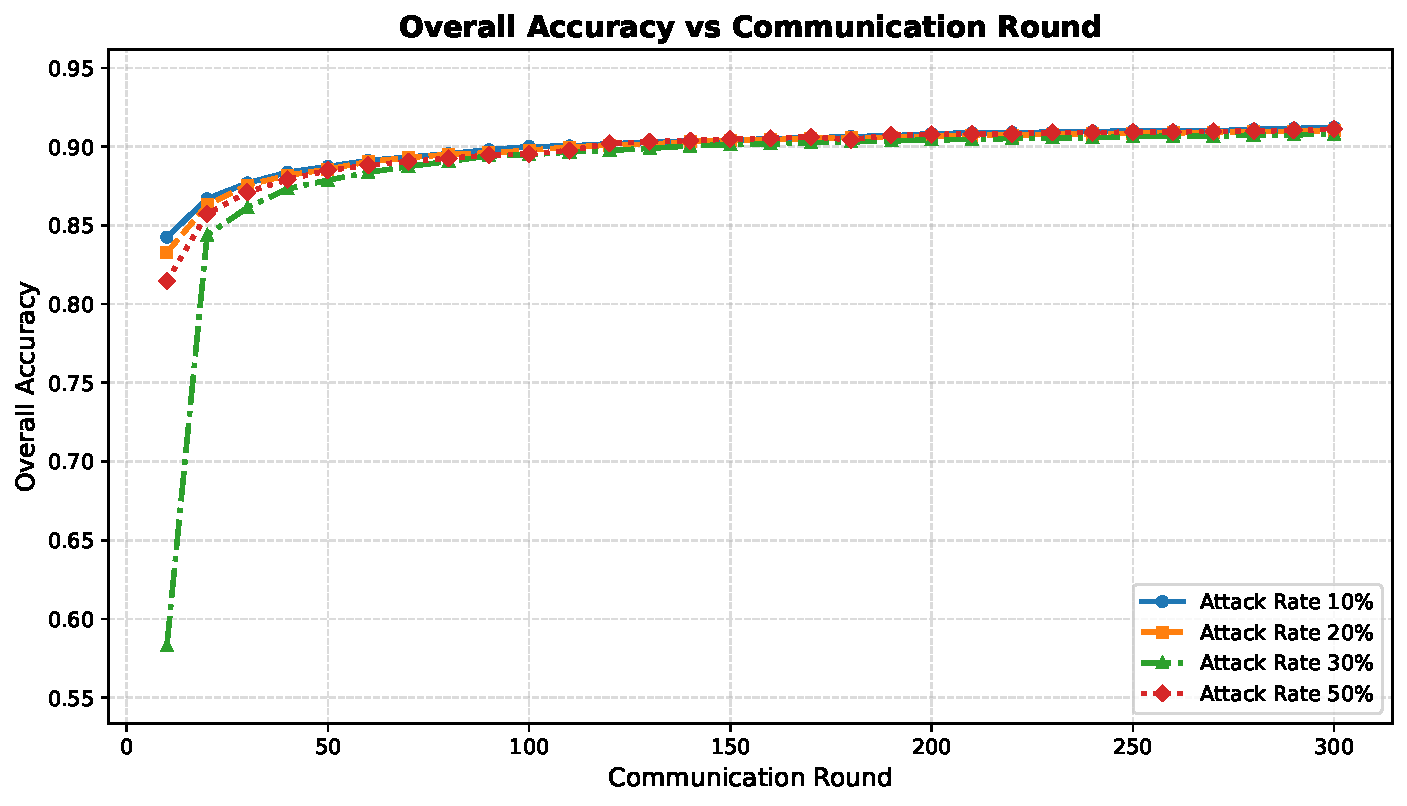
\includegraphics[width=0.47\textwidth]{fig_noniid_untargeted_mnist_acc.pdf}}
\hfill
\subfigure[KDDCup99 ACC trajectory]{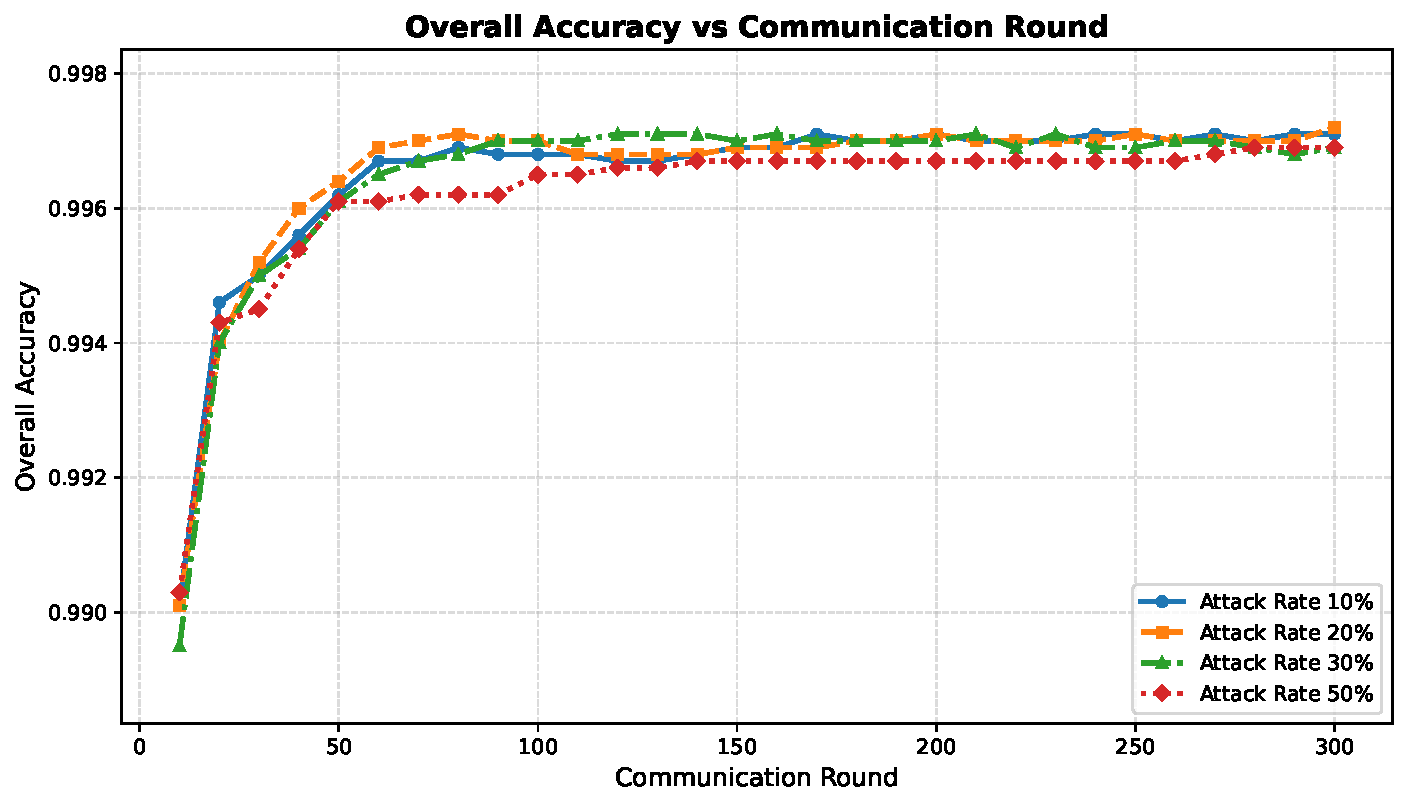
\includegraphics[width=0.47\textwidth]{fig_noniid_untargeted_kdd_acc.pdf}}
\vspace{0.4em}
\subfigure[MNIST malicious-client TPR]{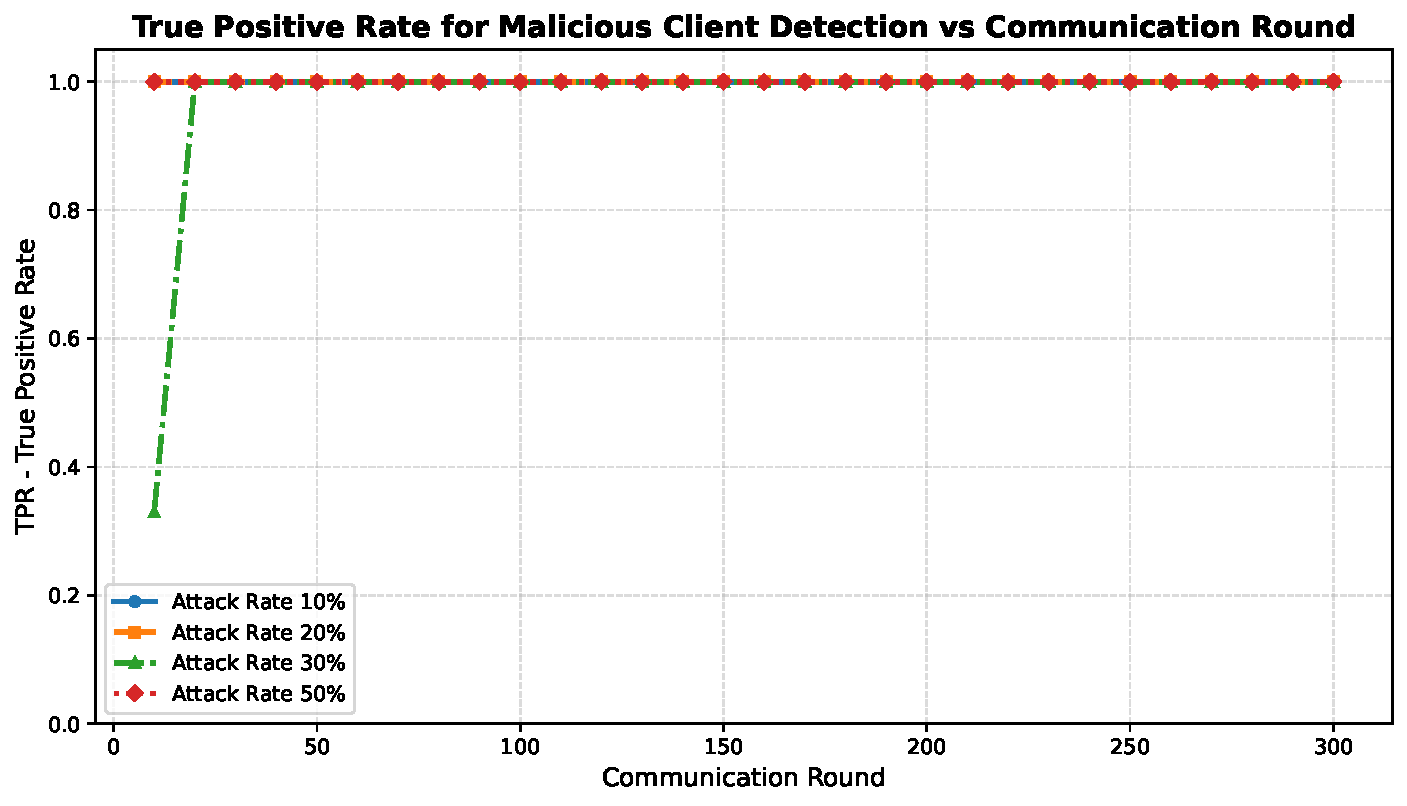
\includegraphics[width=0.47\textwidth]{fig_noniid_untargeted_mnist_tpr.pdf}}
\hfill
\subfigure[KDDCup99 malicious-client TPR]{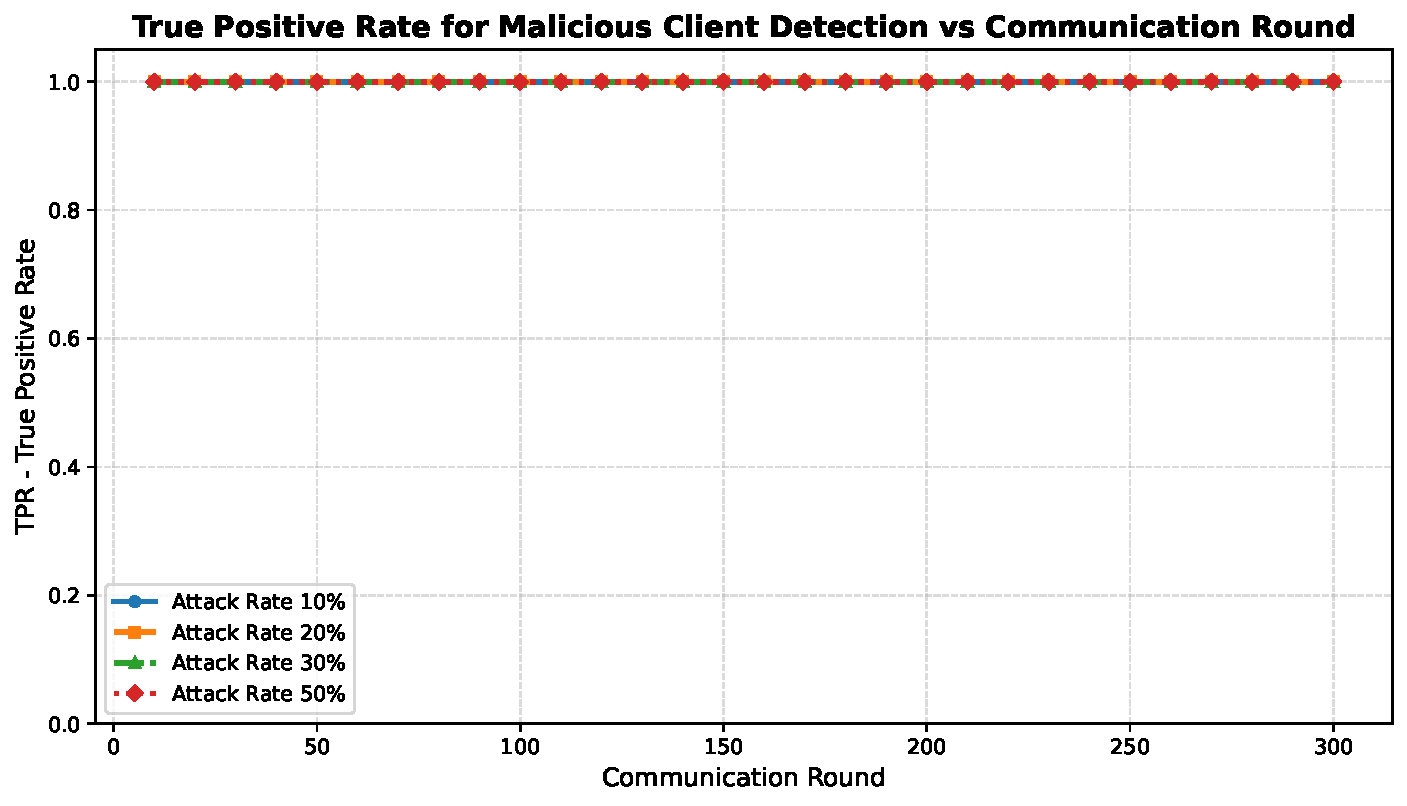
\includegraphics[width=0.47\textwidth]{fig_noniid_untargeted_kdd_tpr.pdf}}
\caption{Non-IID untargeted attack dynamics over 300 communication rounds. Accuracy converges stably for both datasets, while the direction/magnitude audit reaches perfect malicious-client detection by the final round.}
\label{fig:res-noniid-untargeted-dynamics}
\end{figure}

%=====================================================================
\section{Non-IID Partition, Targeted Attacks}
\label{sec:res-nonIID-targ}

A targeted label-flipping attack is a more delicate kind of poisoning than the untargeted case. It tries to break one specific source class while letting the global accuracy stay believable, so reading ACC alone would actively hide the damage. The number that matters here is the target-class accuracy $T_{\text{acc}}$.

\subsection{MNIST}
\label{sec:res-nonIID-targ-mnist}

\begin{table}[H]
\centering
\caption{MNIST, non-IID, targeted label-flipping attack $(c_s=0,c_t=7)$; SenSys 2026 headline targeted-accuracy cell.}
\label{tab:res-nonIID-targ-mnist}
\begin{tabular}{@{}cccc@{}}
\toprule
\textbf{AR} & \textbf{Undefended (\%)} & \textbf{Auditor-based (\%)} & \textbf{FIP-FL (\%)} \\
\midrule
50\% & $\approx 7.00$ & 96.50 & 97.69 \\
\bottomrule
\end{tabular}
\end{table}

\subsection{KDDCup99}
\label{sec:res-nonIID-targ-kdd}

\begin{table}[H]
\centering
\caption{KDDCup99, non-IID partition (2 shards/client), targeted label-flipping attack.}
\label{tab:res-nonIID-targ-kdd}
\begin{tabular}{@{}cccccc@{}}
\toprule
\textbf{AR} & \textbf{ACC (\%)} & \textbf{$T_{\text{acc}}$ (\%)} & \textbf{$O_{\text{acc}}$ (\%)} & \textbf{TPR} & \textbf{FPR} \\
\midrule
10\% & 99.54 & 99.75 & 63.46 & 1.00 & 0.00 \\
20\% & 99.69 & 99.65 & 78.85 & 1.00 & 0.00 \\
30\% & 99.70 & 99.50 & 82.69 & 1.00 & 0.00 \\
50\% & 99.52 & 98.41 & 86.54 & 1.00 & 0.00 \\
\bottomrule
\end{tabular}
\end{table}

\paragraph{Observations.} The MNIST row is the headline cell from the accepted SenSys 2026 poster. With $50\%$ of the clients turning malicious, FIP-FL pushes $T_{\text{acc}}$ from roughly $7\%$ in the undefended run all the way up to $97.69\%$ --- a number that sits above the $96.5\%$ reported by the auditor-based scheme of Yazdinejad et al.~\cite{yazdinejad2024robust}. KDDCup99 follows the same detection pattern across the full attack-rate sweep, with no false positives anywhere in the table and $T_{\text{acc}}=98.41\%$ even at the $50\%$ row.

\begin{figure}[!htbp]
\centering
\subfigure[Target-class accuracy trajectory]{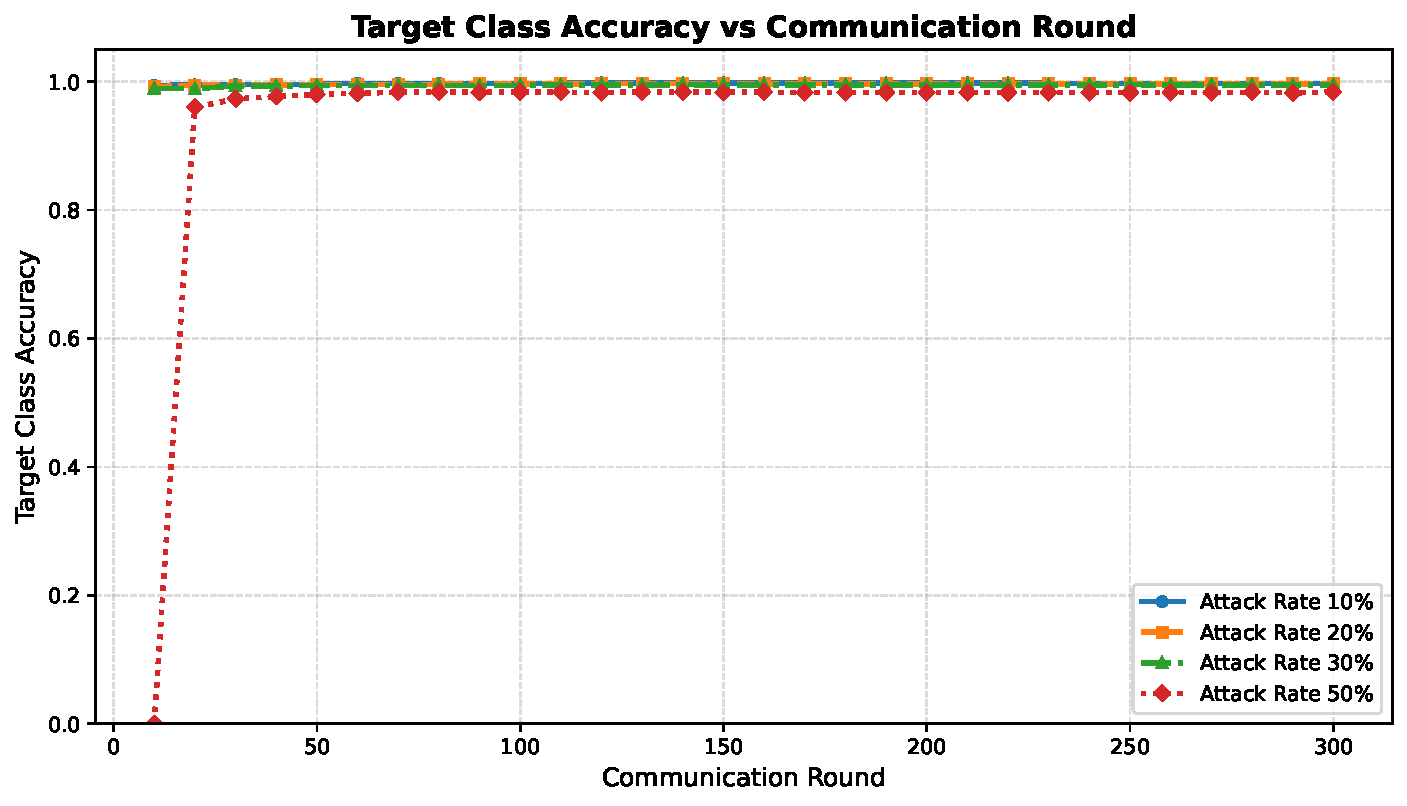
\includegraphics[width=0.47\textwidth]{fig_noniid_targeted_kdd_tacc.pdf}}
\hfill
\subfigure[Round-300 accuracy comparison]{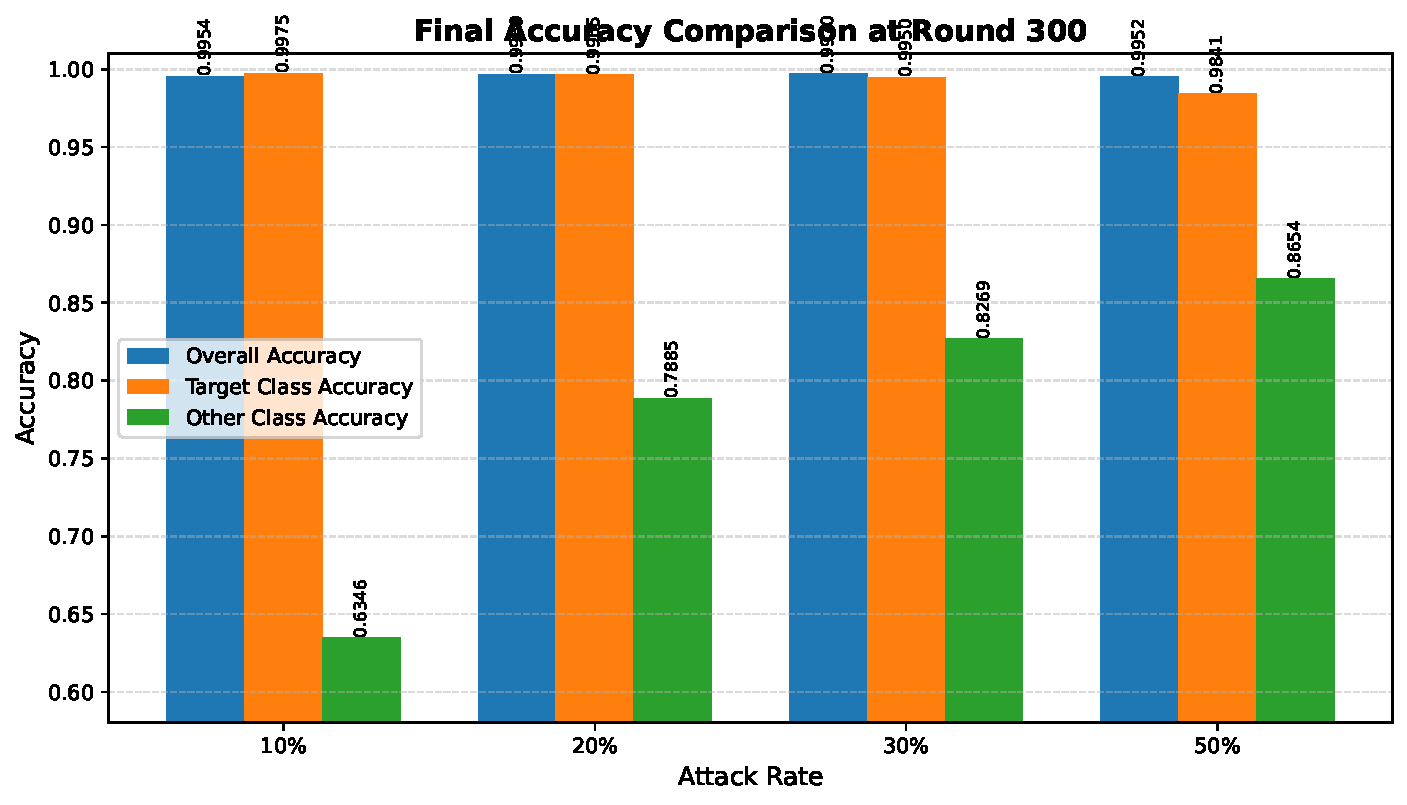
\includegraphics[width=0.47\textwidth]{fig_noniid_targeted_kdd_final_acc.pdf}}
\caption{KDDCup99 non-IID targeted attack results. The target-class trajectory remains high through training, and the round-300 comparison shows that overall and target-class accuracy stay stable even as the malicious-client fraction increases.}
\label{fig:res-noniid-targeted-kdd-dynamics}
\end{figure}

%=====================================================================
\section{IID Partition, Untargeted Attacks}
\label{sec:res-IID-untarg}

The IID rows are included mostly as a sanity-check baseline. With IID partitions the honest clients are statistically very close to one another, which means the distribution of FIP scores in any given round is comparatively tight, and detection should be the easiest setting we will see.

\subsection{MNIST}
\label{sec:res-IID-untarg-mnist}

\begin{table}[H]
\centering
\caption{MNIST, IID partition, untargeted label-flipping attack.}
\label{tab:res-IID-untarg-mnist}
\begin{tabular}{@{}cccccc@{}}
\toprule
\textbf{AR} & \textbf{ACC (\%)} & \textbf{$T_{\text{acc}}$ (\%)} & \textbf{$O_{\text{acc}}$ (\%)} & \textbf{TPR} & \textbf{FPR} \\
\midrule
10\% & 91.49 & 97.51 & 90.40 & 1.00 & 0.00 \\
20\% & 91.50 & 97.51 & 90.39 & 1.00 & 0.00 \\
30\% & 91.33 & 97.42 & 90.28 & 1.00 & 0.00 \\
50\% & 91.32 & 97.42 & 90.22 & 1.00 & 0.00 \\
\bottomrule
\end{tabular}
\end{table}

\subsection{KDDCup99}
\label{sec:res-IID-untarg-kdd}

\begin{table}[H]
\centering
\caption{KDDCup99, IID partition, untargeted label-flipping attack.}
\label{tab:res-IID-untarg-kdd}
\begin{tabular}{@{}cccccc@{}}
\toprule
\textbf{AR} & \textbf{ACC (\%)} & \textbf{$T_{\text{acc}}$ (\%)} & \textbf{$O_{\text{acc}}$ (\%)} & \textbf{TPR} & \textbf{FPR} \\
\midrule
10\% & 99.74 & 99.60 & 85.58 & 1.00 & 0.00 \\
20\% & 99.73 & 99.55 & 85.58 & 1.00 & 0.00 \\
30\% & 99.75 & 99.60 & 85.58 & 1.00 & 0.00 \\
50\% & 99.73 & 99.55 & 85.58 & 1.00 & 0.00 \\
\bottomrule
\end{tabular}
\end{table}

\paragraph{Observations.} In the IID untargeted setting, detection is essentially exact on both datasets --- every row reports $\mathrm{TPR}=1.00$ together with $\mathrm{FPR}=0.00$. The MNIST ACC moves by less than $0.2$ percentage points across the whole attack-rate sweep, and on KDDCup99 the ACC, $T_{\text{acc}}$, and $O_{\text{acc}}$ values together vary by at most $0.05$ percentage points.

\begin{figure}[!htbp]
\centering
\subfigure[MNIST ACC trajectory]{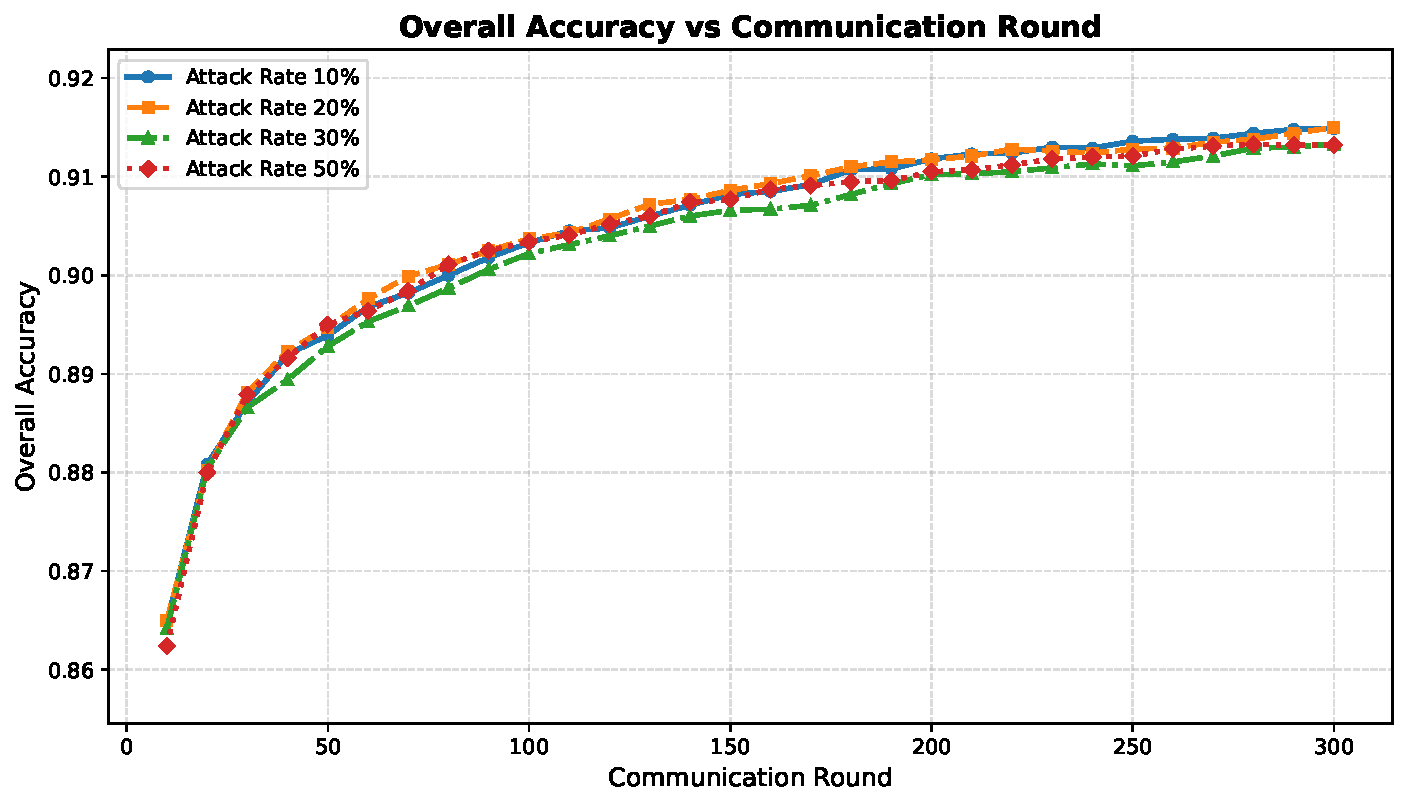
\includegraphics[width=0.47\textwidth]{fig_iid_untargeted_mnist_acc.pdf}}
\hfill
\subfigure[KDDCup99 ACC trajectory]{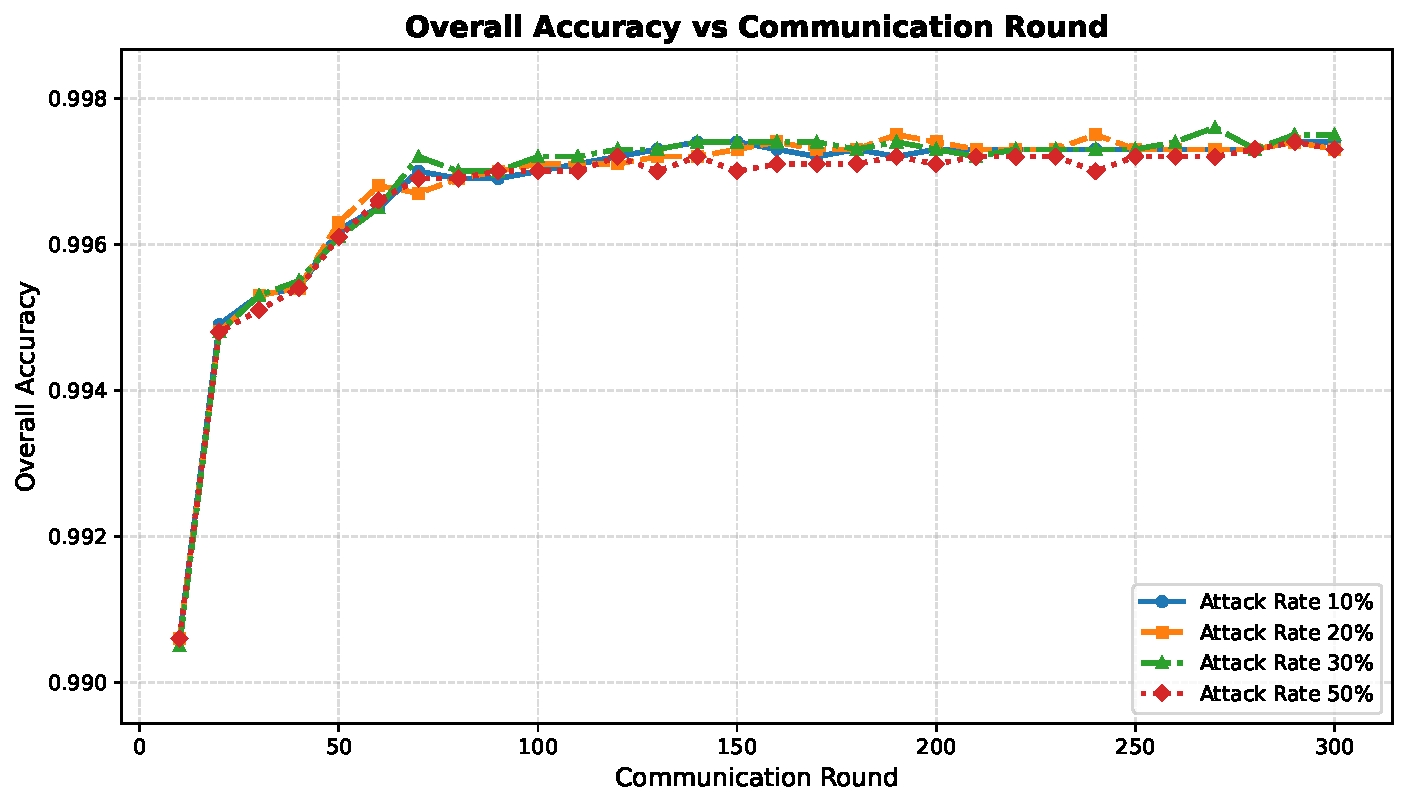
\includegraphics[width=0.47\textwidth]{fig_iid_untargeted_kdd_acc.pdf}}
\vspace{0.4em}
\subfigure[MNIST malicious-client TPR]{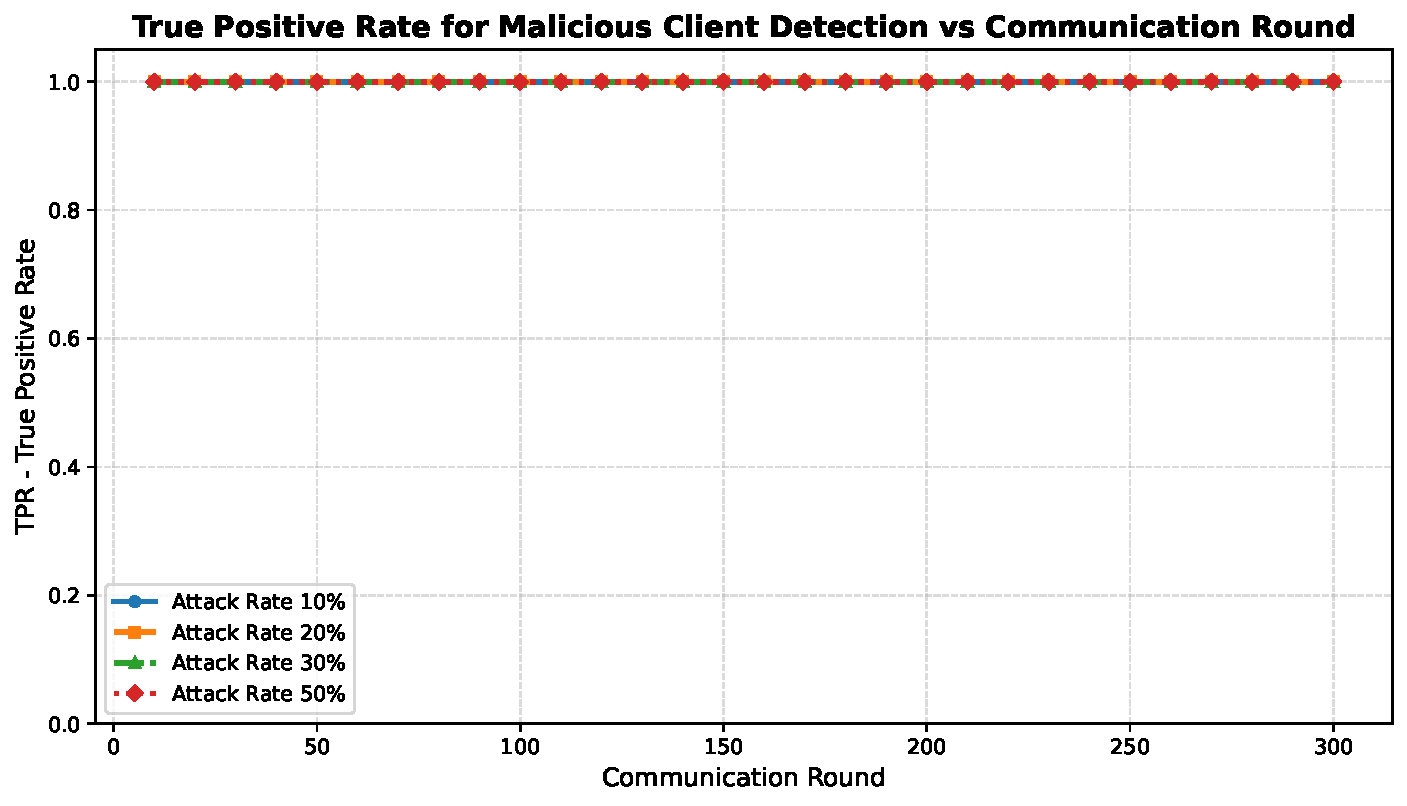
\includegraphics[width=0.47\textwidth]{fig_iid_untargeted_mnist_tpr.pdf}}
\hfill
\subfigure[KDDCup99 malicious-client TPR]{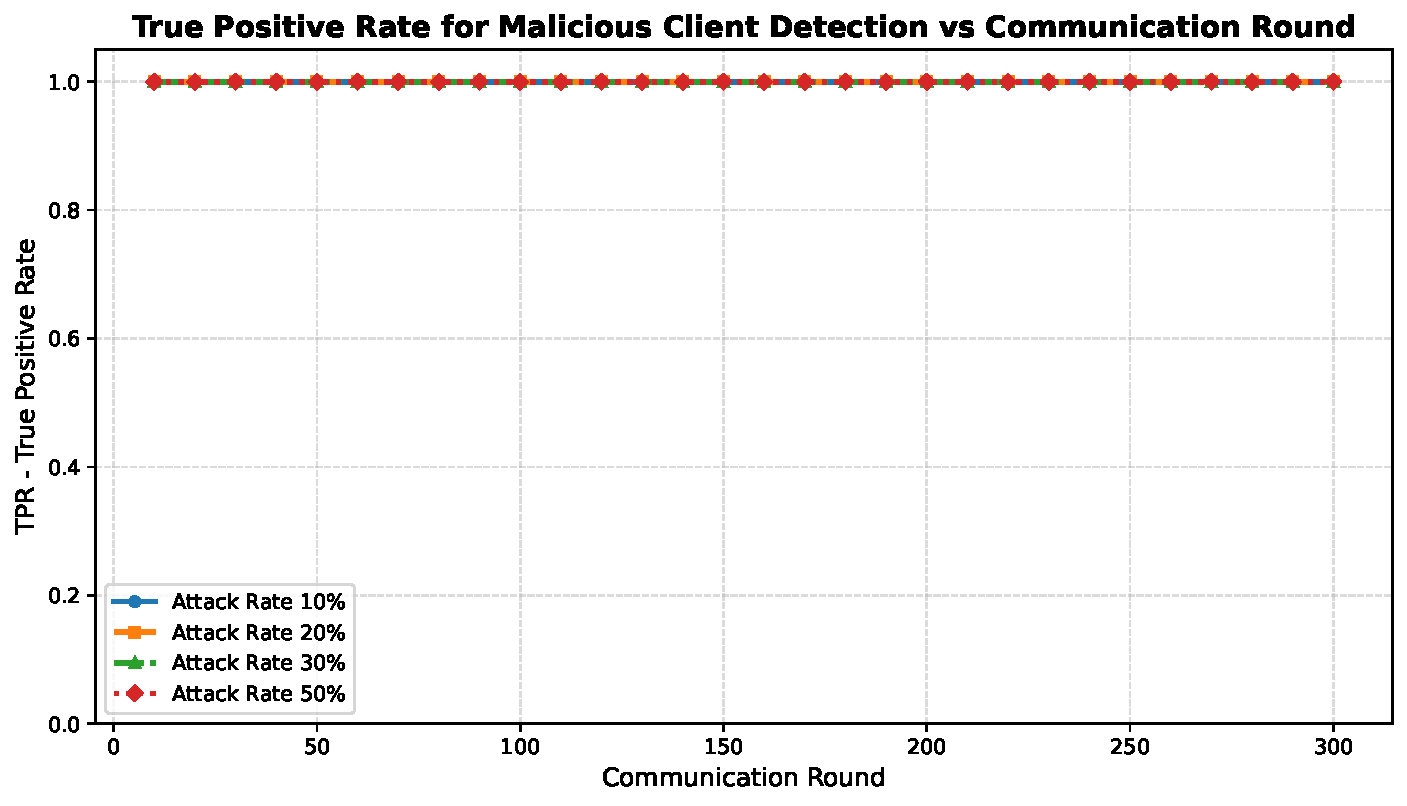
\includegraphics[width=0.47\textwidth]{fig_iid_untargeted_kdd_tpr.pdf}}
\caption{IID untargeted attack dynamics over 300 communication rounds. Both datasets show stable convergence, and the audit maintains perfect malicious-client detection without false positives at the reported final round.}
\label{fig:res-iid-untargeted-dynamics}
\end{figure}

%=====================================================================
\section{IID Partition, Targeted Attacks}
\label{sec:res-IID-targ}

\subsection{MNIST}
\label{sec:res-IID-targ-mnist}

\begin{table}[H]
\centering
\caption{MNIST, IID partition, targeted label-flipping attack $(c_s=0,c_t=7)$.}
\label{tab:res-IID-targ-mnist}
\begin{tabular}{@{}cccccc@{}}
\toprule
\textbf{AR} & \textbf{ACC (\%)} & \textbf{$T_{\text{acc}}$ (\%)} & \textbf{$O_{\text{acc}}$ (\%)} & \textbf{TPR} & \textbf{FPR} \\
\midrule
10\% & 91.62 & 97.51 & 90.57 & 1.00 & 0.00 \\
20\% & 91.42 & 97.42 & 90.35 & 1.00 & 0.00 \\
30\% & 91.32 & 97.42 & 90.22 & 1.00 & 0.00 \\
50\% & 91.43 & 97.42 & 90.35 & 1.00 & 0.00 \\
\bottomrule
\end{tabular}
\end{table}

\subsection{KDDCup99}
\label{sec:res-IID-targ-kdd}

\begin{table}[H]
\centering
\caption{KDDCup99, IID partition, targeted label-flipping attack.}
\label{tab:res-IID-targ-kdd}
\begin{tabular}{@{}cccccc@{}}
\toprule
\textbf{AR} & \textbf{ACC (\%)} & \textbf{$T_{\text{acc}}$ (\%)} & \textbf{$O_{\text{acc}}$ (\%)} & \textbf{TPR} & \textbf{FPR} \\
\midrule
10\% & 99.73 & 99.60 & 84.62 & 1.00 & 0.00 \\
20\% & 99.73 & 99.55 & 85.58 & 1.00 & 0.00 \\
30\% & 99.72 & 99.50 & 85.58 & 1.00 & 0.00 \\
50\% & 99.73 & 99.55 & 85.58 & 1.00 & 0.00 \\
\bottomrule
\end{tabular}
\end{table}

\paragraph{Observations.} The IID targeted case lines up cleanly with the IID untargeted one. Detection stays perfect, false rejections never happen, and the target-class accuracy stays flat across all attack rates. MNIST holds $T_{\text{acc}}\ge97.42\%$ across the table, and KDDCup99 keeps ACC in the $99.72\%$--$99.73\%$ band with $T_{\text{acc}}\ge99.50\%$ on every row.

\begin{figure}[H]
\centering
\subfigure[MNIST target-class accuracy]{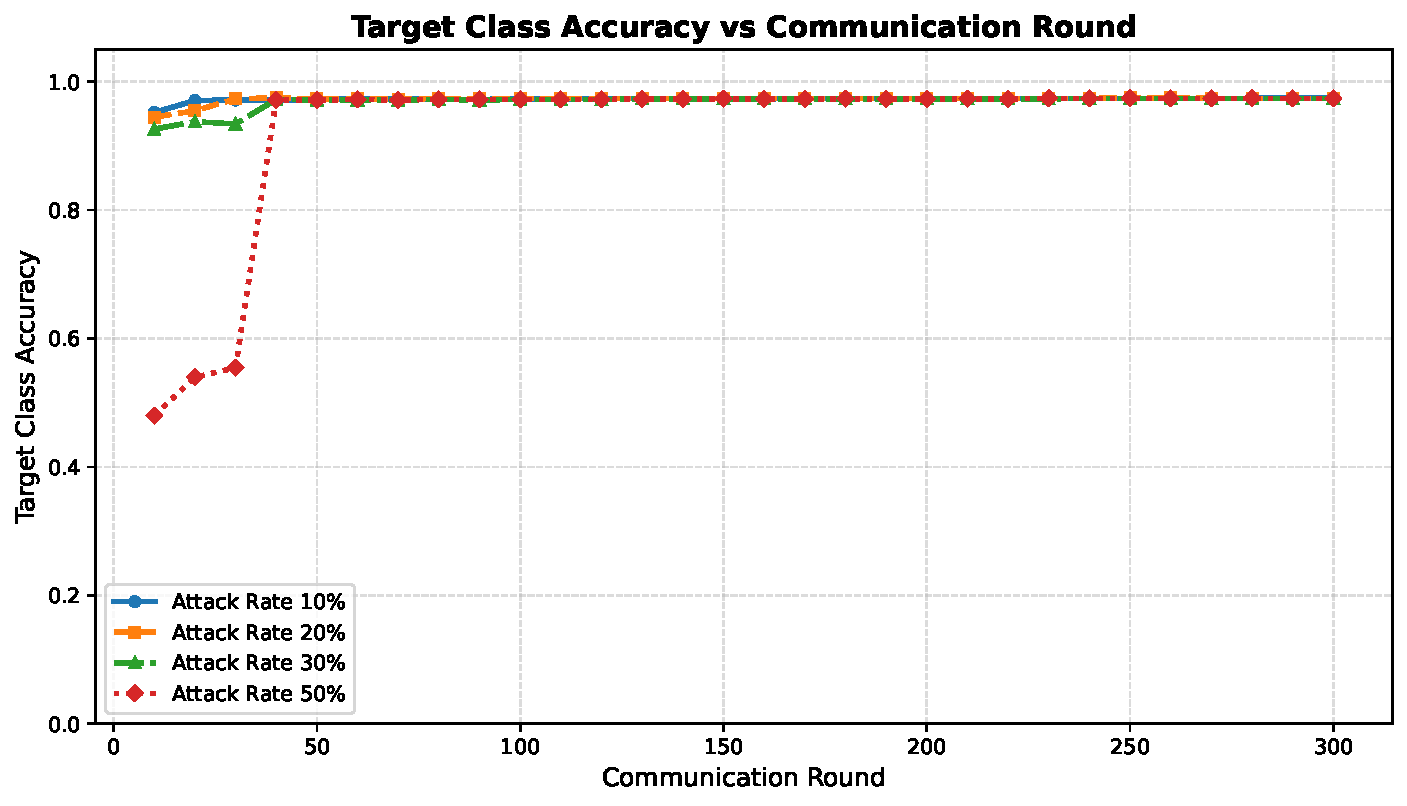
\includegraphics[width=0.47\textwidth]{fig_iid_targeted_mnist_tacc.pdf}}
\hfill
\subfigure[KDDCup99 target-class accuracy]{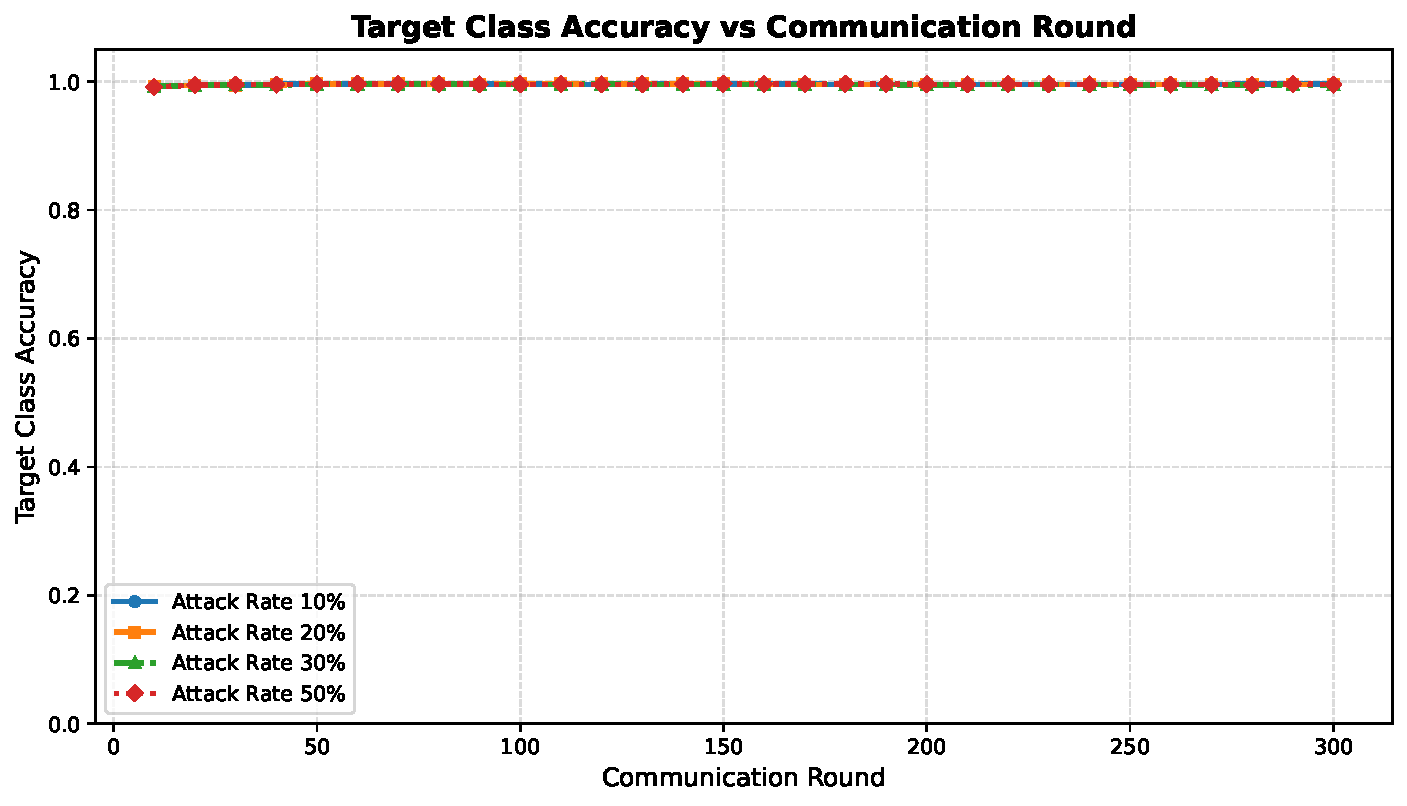
\includegraphics[width=0.47\textwidth]{fig_iid_targeted_kdd_tacc.pdf}}
\caption{IID targeted attack target-class accuracy over 300 communication rounds. In both datasets, the target class recovers to a stable high-accuracy regime by the final round.}
\label{fig:res-iid-targeted-dynamics}
\end{figure}

%=====================================================================
\section{Aggregate Findings Across the Grid}
\label{sec:res-aggregate}

Stepping back from the individual tables, the grid as a whole supports three conclusions. First, every completed row reports $\mathrm{TPR}=1.00$, including the $50\%$ malicious-client cases on both datasets. Second, false rejection only shows up under the heaviest non-IID untargeted load --- exactly the regime where the honest gradients are already pulled apart by label skew --- and even there ACC remains numerically stable. Third, targeted attacks are caught just as reliably as untargeted ones, which suggests that a one-dimensional FIP score against the trusted reference is genuinely sufficient for the poisoning regimes evaluated here. Chapter~\ref{Comparison:chap:chap8} puts these numbers next to the auditor-based baseline.

	\chapter{Comparative Analysis}
\label{Comparison:chap:chap8}
\graphicspath{{17.Chapter8/Images/}}
\raggedbottom

This chapter places FIP-FL alongside the Byzantine-resilient FL defences that were already covered in Chapter~\ref{Literature:chap:chap3}, with the auditor-based baseline of Yazdinejad et al.~\cite{yazdinejad2024robust} taking centre stage. The comparison runs over six axes, privacy leakage, computation, communication, robustness under non-IID skew, engineering cost, and the canonical MNIST non-IID targeted benchmark.

\section{Privacy}
\label{sec:comp-privacy}

The auditor-based scheme has to decrypt cluster-level statistics every round: a projected Gaussian-mixture model along with the Mahalanobis-distance statistics that the filter uses. Even though no individual gradient is ever reconstructed, the cluster means and covariances themselves still leak structural information about the client population. In a non-IID deployment, those statistics can correlate with demographics, hospital specialisation, keyboard language, or any number of other sensitive client traits.

FIP-FL is much more spare. The only thing decrypted per client per round is the scalar FIP score $s_i^{(t)}=\langle \mathbf{g}_i^{(t)},\mathbf{R}^{(t)}\rangle$. There are no cluster means, no covariance matrices, no projection coefficients, no pairwise distances. The privacy improvement is categorical rather than incremental: the verifier sees a single alignment number, and the model update is still derived only from an aggregate.

\section{Computational Complexity}
\label{sec:comp-compute}

\begin{table}[H]
\centering
\caption{Per-round computational cost. $N$: clients; $|\mathcal{A}|$: accepted clients; $d$: model dimension; $B$: batch size; $E$: local epochs.}
\label{tab:comp-computation}
\begin{tabular}{@{}lll@{}}
\toprule
\textbf{Entity} & \textbf{Auditor-based~\cite{yazdinejad2024robust}} & \textbf{FIP-FL} \\
\midrule
Client              & $\mathcal{O}(dBE)$ & $\mathcal{O}(dBE)$ \\
Verifier / Auditor  & $\mathcal{O}(NKD+Nd\log d)+\mathcal{O}(d^3)$ & $\mathcal{O}(Nd+N\log N)$ \\
Aggregation Server  & $\mathcal{O}(dN\log N)$ & $\mathcal{O}(|\mathcal{A}|d)$ \\
\bottomrule
\end{tabular}
\end{table}

\subsection{Time-Complexity Interpretation}
\label{sec:comp-time-interpretation}

The computational comparison in Table~\ref{tab:comp-computation} shows that the main saving of FIP-FL appears at the verifier stage. The client-side cost remains unchanged because both schemes require each client to perform ordinary local SGD on its own data. The difference lies in how the submitted updates are verified and aggregated after local training.

\noindent\textbf{Client-side training.}
The auditor-based PPFL scheme and FIP-FL both have client-side complexity $\mathcal{O}(dBE)$. Both schemes have the same local learning cost because each client trains on mini-batches for $E$ local epochs.

\noindent\textbf{Verification basis.}
The auditor-based PPFL scheme verifies updates through distributional modelling of submitted gradient statistics, while FIP-FL verifies updates through scalar alignment with the bootstrap reference direction. FIP-FL reduces verification from high-dimensional distributional analysis to one scalar score per client.

\noindent\textbf{Verifier / Auditor operations.}
The auditor-based scheme uses projection, Gaussian-mixture modelling, Mahalanobis-distance scoring, and covariance-related computation. FIP-FL uses homomorphic functional inner product computation and bootstrap score filtering. The auditor-based scheme performs richer statistical modelling, whereas FIP-FL performs one encrypted inner product per client.

\noindent\textbf{Verifier / Auditor complexity.}
The auditor-based verifier has complexity $\mathcal{O}(NKD+Nd\log d)+\mathcal{O}(d^3)$, while the FIP-FL verifier has complexity $\mathcal{O}(Nd+N\log N)$. Under the asymptotic model used in this thesis, the additional $\mathcal{O}(d^3)$ term accounts for covariance-inversion style computation in the auditor-side distributional model.

\noindent\textbf{Aggregation cost.}
The auditor-based aggregation cost is $\mathcal{O}(dN\log N)$, while the FIP-FL aggregation cost is $\mathcal{O}(|\mathcal{A}^{(t)}|d)$. FIP-FL aggregates only the accepted ciphertexts after verification, while rejected ciphertexts are dropped.

\noindent\textbf{Scalability implication.}
In the auditor-based PPFL scheme, cost increases with distributional modelling and covariance-related computation. In FIP-FL, verification is linear in the model dimension at the verifier stage. FIP-FL is therefore more scalable for high-dimensional updates because verification avoids cluster-level statistics and covariance estimation.

Here, $N$ is the number of clients, $d$ is the model dimension, $B$ is the batch size, $E$ is the number of local epochs, $K$ is the number of mixture components, $D$ is the auditor-side feature or projection dimension, and $\mathcal{A}^{(t)}$ is the accepted client set in round $t$.

Overall, this comparison shows that FIP-FL keeps the same client-side learning cost as the auditor-based baseline but replaces auditor-side distributional modelling with a scalar encrypted inner-product audit. For each client, the verifier computes one homomorphic functional inner product with the fixed bootstrap reference direction, giving $\mathcal{O}(Nd)$ score-computation cost. The bootstrap audit then filters scalar scores, contributing $\mathcal{O}(N\log N)$. After verification, only accepted ciphertexts are aggregated, giving $\mathcal{O}(|\mathcal{A}^{(t)}|d)$. Thus, FIP-FL shifts verification from high-dimensional statistical auditing to linear-time encrypted alignment testing, making the verifier stage easier to scale and parallelise across clients.

\section{Communication Complexity}
\label{sec:comp-comm}

\begin{table}[H]
\centering
\caption{Per-round communication cost by directed link.}
\label{tab:comp-comm}
\begin{tabular}{@{}lll@{}}
\toprule
\textbf{Link} & \textbf{Auditor-based~\cite{yazdinejad2024robust}} & \textbf{FIP-FL} \\
\midrule
Client $\to$ Verifier & $\mathcal{O}(Nd)$ & $\mathcal{O}(Nd)$ \\
Verifier $\to$ Server & $\mathcal{O}(L(Z+N))$ & $\mathcal{O}(|\mathcal{A}|d)$ \\
Server $\to$ Clients  & $\mathcal{O}(d)$ & $\mathcal{O}(d)$ \\
\bottomrule
\end{tabular}
\end{table}

The first leg of communication, the client-to-verifier payload, is the same in both designs, since both schemes need the encrypted updates to reach the verifier somehow. The savings show up after the audit. FIP-FL never forwards a rejected ciphertext, so the verifier-to-server traffic shrinks with the rejection rate, and the extra auditor-to-server hop that the auditor-based pipeline relies on simply does not exist here.

\section{Robustness and Engineering Trade-Offs}
\label{sec:comp-robust-engineering}

The detector inside the auditor-based scheme leans on the assumption that the honest-client cluster is both tighter and more populous than the malicious cluster, an assumption that gets noticeably weaker once label skew is in the mix. FIP-FL takes a different tack: it tests, for each individual update, whether the update is aligned with the trusted reference direction and whether its score passes the bootstrap audit. The whole admissibility check stays one-dimensional, and that one-dimensional behaviour is what carries the audit through the heterogeneous cases.

A useful side-effect of this design is that it limits cascade behaviour after a hard round. Only the updates that clear the bootstrap audit ever enter the aggregate, and the bootstrap reference remains fixed across rounds, which prevents a single noisy round from completely re-orienting the audit. The Phase~II FIP computations are independent across clients, so they parallelise cleanly, on the 25-core workstation described in Section~\ref{sec:setup-impl} this gave a wall-clock speed-up of about $13\times$. The single-reference design also avoids the extra homomorphic inner products that a multi-reference cone would have demanded.

\section{Scheme-versus-Scheme Accuracy Comparison}
\label{sec:comp-accuracy}

\begin{table}[H]
\centering
\caption{Accuracy on MNIST non-IID under a $50\%$ malicious-client rate. Entries are percentages; baseline values are from~\cite{yazdinejad2024robust}.}
\label{tab:comp-accuracy}
\begin{tabular}{@{}lcc@{}}
\toprule
\textbf{Scheme} & \shortstack{\textbf{Targeted}\\\textbf{target-class accuracy}\\\textbf{($T_{\text{acc}}$)}} & \shortstack{\textbf{Untargeted}\\\textbf{overall accuracy}\\\textbf{(ACC)}} \\
\midrule
Krum~\cite{blanchard2017machine}              & 71.4 & 78.3 \\
Auror~\cite{shen2016auror}                    & 32.5 & 49.9 \\
PEFL~\cite{liu2021privacy}                    & 46.4 & 57.4 \\
Sybils / FoolsGold~\cite{fung2020limitations} & 89.7 & 89.5 \\
FL-Trust~\cite{cao2021fltrust}                & 37.8 & 43.4 \\
ShieldFL~\cite{ma2022shieldfl}                & 90.1 & 89.4 \\
Auditor-based~\cite{yazdinejad2024robust}     & 96.5 & 96.3 \\
\midrule
\textbf{FIP-FL (this thesis)}                 & \textbf{97.69} & 88.82 \\
\bottomrule
\end{tabular}
\end{table}

In the table above, FIP-FL records the best target-class accuracy ($T_{\text{acc}}$) of every targeted entry, and it does so while resting on weaker trust assumptions than the auditor-based row. Its untargeted overall accuracy (ACC) is competitive with FoolsGold and ShieldFL but does not quite reach the auditor-based result, and that gap is the clearest empirical place where future work could push further. For the purposes of this thesis the relevant point is the qualitative one: FIP-FL produces the strongest target-class recovery without decrypting any cluster statistics and without bringing in an external auditor.

	\chapter{Conclusion and Future Work}
\label{Conclusion:chap:chap9}
\graphicspath{{18.Chapter9/Images/}}
\raggedbottom

\section{Summary of the Thesis}
\label{sec:concl-summary}

The argument the thesis has been making is, in one line, that Byzantine-resilient privacy-preserving federated learning does not actually need an external auditor to decrypt cluster-level structure. FIP-FL swaps that trust anchor for a functional inner product taken between each encrypted client update and a fixed bootstrap trusted reference direction. The single scalar that the inner product produces is what feeds the bootstrap audit, whose direction test catches label-flip style reversals.

The proposed approach is implemented through a simple pipeline. Paillier encryption is used at the cryptographic layer, the verifier computes client scores homomorphically, the server aggregates only the accepted encrypted updates, and the bootstrap reference direction remains fixed across rounds. The theoretical analysis lines up with this design, scalar-gradient privacy, a bootstrap audit rejection rule for malicious updates, and a monotone loss-decrease under $L$-smoothness. Empirically, FIP-FL ends up detecting every malicious-client configuration in the completed grid, lifts MNIST non-IID target-class accuracy from roughly $7\%$ in the undefended baseline to $97.69\%$ at a $50\%$ malicious-client rate, and replaces the auditor's $\mathcal{O}(d^3)$ covariance-inversion step with a verification stage that parallelises to a $13\times$ wall-clock speed-up in Phase~II.

\section{Limitations and Future Work}
\label{sec:concl-limits-future}

The main limitations of this thesis arise from the experimental setting. FIP-FL is evaluated using softmax logistic regression models, parameter dimensions in the low-thousand range, a fixed client population, and a single attack type in each run.

Extending the method to deep networks will likely require packed homomorphic encryption schemes such as BFV or CKKS~\cite{cheon2017homomorphic}. A more realistic setting should also consider client churn, evolving data distributions, adaptive adversaries, and combined attack strategies such as label flipping together with update scaling.

Another limitation concerns the initialization of the reference direction. In the current design, this direction is derived from a small public dataset. Although this works well in the present experiments, it assumes the availability of such public data.

A stronger approach for the first round would be to estimate the reference direction from robust aggregate statistics computed over the clients themselves, while still avoiding decryption of individual gradients. Beyond this, FIP-FL should be evaluated on real laptop, mobile, and edge devices to better understand the trade-off among encryption overhead, communication cost, and model utility in practical privacy-preserving federated learning settings.

	\endgroup
	
	%
	\singlespacing
	\bibliographystyle{unsrtnat}
	\bibliography{references}

	
	
\end{document}
